\documentclass[a4paper,12pt]{book}
\usepackage{polski}
\usepackage{float}
\usepackage[utf8]{inputenc}
\usepackage[T1]{fontenc}  
\usepackage[margin=1in,left=1.5in,includefoot]{geometry}
\usepackage{fancyhdr}
\usepackage{wrapfig}
\usepackage{amsmath,amsfonts,amssymb,amsthm}
\usepackage[british,polish]{babel} 
\usepackage{indentfirst}
\usepackage{lmodern}
\usepackage{graphicx} 
\usepackage{hyperref}
\usepackage{booktabs}
\usepackage{tikz}
\usepackage{pgfplots}
\usepackage{mathtools}
\usepackage{geometry}
\usepackage{listings}
\pagestyle{fancy}
\usepackage{graphicx}
\usepackage{cite}
\graphicspath{ {./images/} }
\usepackage[page]{appendix} % toc,
\renewcommand{\appendixtocname}{Dodatki}
\renewcommand{\appendixpagename}{Dodatki}
\renewcommand{\appendixname}{Dodatek}
%%%%%%%%%%%% ZYWA PAGINA %%%%%%%%%%%%%%%
% brak kapitalizacji zywej paginy
\usepackage{fancyhdr}
\pagestyle{fancy}
\fancyhf{}
\fancyhead[LO]{\nouppercase{\it\rightmark}}
\fancyhead[RE]{\nouppercase{\it\leftmark}}
\fancyhead[LE,RO]{\it\thepage}


\fancypagestyle{tylkoNumeryStron}{%
   \fancyhf{} 
   \fancyhead[LE,RO]{\it\thepage}
}

\fancypagestyle{NumeryStronNazwyRozdzialow}{%
   \fancyhf{} 
   \fancyhead[LO]{\nouppercase{\it\rightmark}}
   \fancyhead[RE]{\nouppercase{\it\leftmark}}
   \fancyhead[LE,RO]{\it\thepage}
}
\newcounter{stronyPozaNumeracja}

\newcommand{\hcancel}[1]{%
    \tikz[baseline=(tocancel.base)]{
        \node[inner sep=0pt,outer sep=0pt] (tocancel) {#1};
        \draw[red] (tocancel.south west) -- (tocancel.north east);
    }%
}%


\lstdefinelanguage[ECMAScript2015]{JavaScript}[]{JavaScript}{
  morekeywords=[1]{await, async, case, catch, class, const, default, do,
    enum, export, extends, finally, from, implements, import, instanceof,
    let, static, super, switch, throw, try},
  morestring=[b]` % Interpolation strings.
}


%
% JavaScript version 1.1 by Gary Hammock
%
% Reference:
%   B. Eich and C. Rand Mckinney, "JavaScript Language Specification
%     (Preliminary Draft)", JavaScript 1.1.  1996-11-18.  [Online]
%     http://hepunx.rl.ac.uk/~adye/jsspec11/titlepg2.htm
%

\lstdefinelanguage{JavaScript}{
  morekeywords=[1]{break, continue, delete, else, for, function, if, in,
    new, return, this, typeof, var, void, while, with,  public, private, protected, constructor, abstract },
  % Literals, primitive types, and reference types.
  morekeywords=[2]{false, null, true, boolean, number, string, undefined,
    Array, Boolean, Date, Math, Number, String, Object},
  % Built-ins.
  morekeywords=[3]{eval, parseInt, parseFloat, escape, unescape, length},
  sensitive,
  morecomment=[s]{/*}{*/},
  morecomment=[l]//,
  morecomment=[s]{/**}{*/}, % JavaDoc style comments
  morestring=[b]',
  morestring=[b]"
}[keywords, comments, strings]


\lstalias[]{ES6}[ECMAScript2015]{JavaScript}

% Requires package: color.
\definecolor{mediumgray}{rgb}{0.3, 0.4, 0.4}
\definecolor{mediumblue}{rgb}{0.0, 0.0, 0.8}
\definecolor{forestgreen}{rgb}{0.13, 0.55, 0.13}
\definecolor{darkviolet}{rgb}{0.58, 0.0, 0.83}
\definecolor{royalblue}{rgb}{0.25, 0.41, 0.88}
\definecolor{crimson}{rgb}{0.86, 0.8, 0.24}

\lstdefinestyle{JSES6Base}{
  backgroundcolor=\color{white},
  basicstyle=\ttfamily,
  breakatwhitespace=false,
  breaklines=false,
  captionpos=b,
  columns=fullflexible,
  commentstyle=\color{mediumgray}\upshape,
  emph={},
  emphstyle=\color{crimson},
  extendedchars=true,  % requires inputenc
  fontadjust=true,
  frame=single,
  identifierstyle=\color{black},
  keepspaces=true,
  keywordstyle=\color{mediumblue},
  keywordstyle={[2]\color{darkviolet}},
  keywordstyle={[3]\color{royalblue}},
  numbers=left,
  numbersep=5pt,
  numberstyle=\tiny\color{black},
  rulecolor=\color{black},
  showlines=true,
  showspaces=false,
  showstringspaces=false,
  showtabs=false,
  stringstyle=\color{forestgreen},
  tabsize=2,
  title=\lstname,
  upquote=true  % requires textcomp
}

\lstdefinestyle{JavaScript}{
  language=JavaScript,
  style=JSES6Base
}
\lstdefinestyle{ES6}{
  language=ES6,
  style=JSES6Base
}

\newcommand{\miesiac}{%
  \ifcase\the\month
  \or styczeń% 1
  \or luty% 2
  \or marzec% 3
  \or kwiecień% 4
  \or maj% 5
  \or czerwiec% 6
  \or lipiec% 7
  \or sierpień% 8
  \or wrzesień% 9
  \or październik% 10
  \or listopad% 11
  \or grudzień% 12
  \fi}


%%%%%%%%%%%%%%%%%%%%%%%%%%%%%%%%%%%%%%%%%%%%%%
% Helvetica font macros for the title page:
\newcommand{\headerfont}{\fontfamily{phv}\fontsize{18}{18}\bfseries\scshape\selectfont}
\newcommand{\titlefont}{\fontfamily{phv}\fontsize{18}{18}\selectfont}
\newcommand{\otherfont}{\fontfamily{phv}\fontsize{14}{14}\selectfont}

%%%%%%%%%%%%%%%%%%%%%%%%%%%%%%%%%%%%%%%%%%%%%%
%%%%%%%%%%%%%%%%%%%%%%%%%%%%%%%%%%%%%%%%%%%%%%
%%%%%%%%%%%%%%%%%%%%%%%%%%%%%%%%%%%%%%%%%%%%%%
%%%%%%%%%%%%%%%%%%%%%%%%%%%%%%%%%%%%%%%%%%%%%%
%%%%%%%%%%%%%%%%%%%%%%%%%%%%%%%%%%%%%%%%%%%%%%
%%%%%%%%%%%%%%%%%%%%%%%%%%%%%%%%%%%%%%%%%%%%%%
%%%%%%%%%%%%%%%%%%%%%%%%%%%%%%%%%%%%%%%%%%%%%%


\newcommand{\autor}{Kamil Susek}
\newcommand{\promotor}{dr inż. Marcin Połomski}
\newcommand{\konsultant}{dr inż. Imię Nazwisko}
\newcommand{\tytul}{Zastosowanie technologii Blockchain w implementacji prostego systemu do głosowania on-line}
\newcommand{\polsl}{Politechnika Śląska}
\newcommand{\wydzial}{Wydział Automatyki, Elektroniki i Informatyki}

\begin{document}

%\kslistofremarks 
	
%%%%%%%%%%%%%%%%%%  STRONA TYTULOWA %%%%%%%%%%%%%%%%%%%
\pagestyle{empty}
{
	\newgeometry{top=2.5cm,%
	             bottom=2.5cm,%
	             left=3cm,
	             right=2.5cm}
	\sffamily
	\rule{0cm}{0cm}
	
	\begin{center}
	
\includegraphics[width=0.4\textwidth]{politechnika_sl_logo_bw_poziom_pl.eps}
	\end{center} 
	\vspace{1cm}
	\begin{center}
	\headerfont \polsl
	\end{center}
	\begin{center}
	\headerfont \wydzial
	\end{center}
	\vfill
	\begin{center}
	\titlefont Praca dyplomowa inżynierska
	\end{center}
	\vfill
	
	\begin{center}
	\otherfont \tytul\par
	\end{center}
	
	\vfill
	
	\vfill
	 
	\noindent\vbox
	{
		\hbox{\otherfont autor: \autor}
		\vspace{12pt}
		\hbox{\otherfont kierujący pracą: \promotor}
		%\vspace{12pt}  % zakomentuj, jezeli nie ma konsultanta
		%\hbox{\otherfont konsultant: \konsultant} % zakomentuj, jezeli nie ma konsultanta
	}
	\vfill 
 
   \begin{center}
   \otherfont Gliwice,  \miesiac\ \the\year
   \end{center}	
	\restoregeometry
}
  

\cleardoublepage

\begin{flushright}
załącznik nr 2 do zarz. nr 97/08/09 
\end{flushright}

\vfill  

\begin{center}
\Large\bfseries Oświadczenie
\end{center}

\vfill

Wyrażam  zgodę / Nie wyrażam zgody*  na  udostępnienie  mojej  pracy  dyplomowej / rozprawy doktorskiej*.

\vfill

Gliwice, dnia \today

\vfill

\rule{0.5\textwidth}{0cm}\dotfill 

\rule{0.5\textwidth}{0cm}
\begin{minipage}{0.45\textwidth}
{\begin{center}(podpis)\end{center}}
\end{minipage} 

\vfill

\rule{0.5\textwidth}{0cm}\dotfill 

\rule{0.5\textwidth}{0cm}
\begin{minipage}{0.45\textwidth}
{\begin{center}\rule{0mm}{5mm}(poświadczenie wiarygodności podpisu przez Dziekanat)\end{center}}
\end{minipage}


\vfill

* podkreślić właściwe

 


%%%%%%%%%%%%%%%%%%%%% oswiadczenie promotora o spełnieniu wymagań formalnych %%%%%%%%%%%%%%%%%%%
\cleardoublepage

\rule{1cm}{0cm}

\vfill  

\begin{center}
\Large\bfseries Oświadczenie promotora
\end{center}

\vfill

Oświadczam, że praca „\tytul” spełnia wymagania formalne pracy dyplomowej inżynierskiej.

\vfill



\vfill

Gliwice, dnia \today

\rule{0.5\textwidth}{0cm}\dotfill 

\rule{0.5\textwidth}{0cm}
\begin{minipage}{0.45\textwidth}
{\begin{center}(podpis promotora)\end{center}}
\end{minipage} 

\vfill

\cleardoublepage

%%%%%%%%%%%%%%%%%% SPIS TRESCI %%%%%%%%%%%%%%%%%%%%%%
\pagenumbering{Roman}
\pagestyle{tylkoNumeryStron}
\tableofcontents

%%%%%%%%%%%%%%%%%%%%%%%%%%%%%%%%%%%%%%%%%%%%%%%%%%%%%
\mainmatter
\pagenumbering{arabic}
\setcounter{stronyPozaNumeracja}{\value{page}}
\pagestyle{NumeryStronNazwyRozdzialow}

%%%%%%%%%%%%%% wlasciwa tresc pracy %%%%%%%%%%%%%%%%%

\chapter{Wstęp}

Rozwój technologii pozwala na tworzenie coraz większych i bardziej bezpiecznych systemów, co prowadzi do przenoszenia niektórych procesów życia społecznego, do świata wirtualnego. Takie działania pozwalają na zwiększenie efektywności i zmniejszenie kosztów tych procesów. Dodatkowo wyeliminowanie wpływu czynnika ludzkiego zwiększa wiarygodność takiego procesu i poprawia bezpieczeństwo. Przykładem takiego procesu jest głosowanie, które w tradycyjnej formie jest czasochłonne i trudne w organizacji. Natomiast przykładem technologii, która doprowadziła do prawdziwej rewolucji jest Blockchain. Blockchain odpowiada za przełomowe rozwiązanie w sektorze finansów, jakim jest Bitcoin, który zapoczątkował rozwój systemów odpowiedzialnych za istotne procesy życia społecznego.

Tematem niniejszej pracy jest głosowanie \textit{on-line}, czyli system głosowania przez internet, który będzie wspierany przez technologię Blockchain. W ramach pracy został przedstawiony teoretyczny model systemu, którego część została zaimplementowana. Do zaimplementowanej części systemu należą: aplikacje internetowe wyborcy oraz organizatora i grupa serwisów dostarczających REST (Representational State Transfer) API (Application Programming Interface). Aplikacja wyborcy pozwala na zalogowanie się, wysłanie głosu i uzyskanie wyników wyborów. Natomiast aplikacja organizatora dostarcza narzędzia do konfiguracji i nadzorowania procesu wyborczego. Dostarczono również możliwość konfigurowania sieci Blockchain, która jest odpowiedzialna za zapisanie i zabezpieczenie dodawanych głosów.

W rozdziale pierwszym zostały przybliżone cele projektu, jego założenia, a także zakres pracy. Rozdział drugi poświęcony jest analizie zagadnienia wchodzącego w skład pracy, jakim jest Blockchain. W tym rozdziale przybliżono koncepcję technologii Blockchain, jej budowę i zastosowania. Rozdział trzeci zawiera przegląd wybranych rozwiązań wyborów \textit{on-line}. W rozdziale czwartym sformułowano wymaganie funkcjonalne i niefunkcjonalne systemu. W tym rozdziale znajdują się informacje teoretyczne dotyczące systemu. W rozdziale czwartym znajdują się również diagramy przypadków użycia i opis wykorzystanych technologii. Rozdział piąty dotyczy specyfikacji zewnętrznej oprogramowania. W tym rodziale zawarto informacje dotyczące instalacji i uruchamiania oprogramowania, a także zrzuty ekranu pokazujące scenariusze działania systemu. Rozdział szósty zawiera informacje dotyczące specyfikacji wewnętrznej. W tym rozdziale znajduje się opis architektury systemu, wykorzystane struktury danych i szczegóły implementacyjne wybranych części systemu. Rozdział szósty zawiera również informacje o wykorzystanych wzorcach projektowych i algorytmach. Rozdział siódmy dotyczy sposobów testowania poszczególnych modułów oprogramowania. Natomiast rozdział ósmy jest podsumowaniem pracy, a w jego skład wchodzą spełnione założenia projektu, napotkane błędy i wnioski.

\section{Cele i założenia pracy}

Celem pracy jest opracowanie oraz zaimplementowanie systemu, który umożliwia przeprowadzenie wyborów przez internet. Głównym założeniem projektu jest wykorzystanie technologii Blockchain. Zakres pracy obejmuje:

\begin{itemize}
	\item analizę dziedziny i przegląd literatury dotyczącej wyborów internetowych i technologii Blockchain,
	\item opracowanie systemu wyborów internetowych od strony teoretycznej,
	\item implementację wybranej części całego systemu,
	\item weryfikację i walidację aplikacji.
\end{itemize}


\chapter{Blockchain}
Podstawy teoretyczne technologii Blockchain powstały już w roku 1991, a zostały opracowane przez dr Stuart'a Haber'a oraz dr W. Scott Stornett'a. Naukowcy zajmowali się opracowaniem systemu, zabezpieczającego cyfrowe dokumenty przed podrobieniem, bądź podmianą. System opierał się na łańcuchach bloków, gdzie w każdym bloku znajdowały się cyfrowe dane dokumentu. Podczas dodawania nowego dokumentu do łańcucha, podpisywano go za pomocą tak zwanego stempla czasu (ang. timestamp), a następnie dokument był łączony z poprzednim dokumentem. Łączenie polega na przypisaniu nowem blokowi, wskaźnika na poprzedni dokument. Wartością wskaźnika były określone dane poprzedniego dokumentu, co stanowiło zabezpieczenie dokumentów. Jeżeli zawartość dokumentu w łańcuchu uległaby zmianie, to należałoby zmienić również wskaźnik na ten dokument\cite{pa}.

Kamieniem milowym w popularyzacji tego pomysłu był open-source'owy projekt o nazwie Bitcoin. Projekt ten powstał w roku 2009, a jego autorstwo przyznawane jest Satoshi'emu Nakamoto. Bitcoin to kryptowaluta, której podstawa działania oparta jest o wykorzystanie systemu Blockchain. Transakcje wykonane za pomocą Bitcoin'a zapisywane są na tak zwanym arkuszu, który jest widoczny dla każdego uczestnika sieci. Blockchain odgrywa swoją rolę w rejestrowaniu nowych transakcji i zapisywaniu ich w arkuszu. Arkusz ma strukturę łańcucha bloków, a sama architektura Blockchain została ulepszona o działanie w rozproszonej sieci \textit{Peer to Peer}. \textit{Peer to Peer} pozwala na udostępnienie zawartości Bitcoin'a milionom użytkowników na całym świecie, a dodatkowo zabezpieczenie sieci. Bitcoin wykorzystuje algorytm konsensusu, w celu zapewnienia spójności zawartości węzłów sieci. Jest to algorytm o nazwie \textit{Proof of Work}, który odpowiada za silnie kojarzony z Bitcoin'em proces tzw. \textit{"kopania Bitcoinów"}.
Działanie \textit{Proof of Work} polega na wkładzie odpowiedniej ilości mocy obliczeniowej przez węzły sieci, poprzez rozwiązanie zagadki matematycznej, w celu utworzenia nowego bloku. Węzeł który rozwiąże zagadkę jako pierwszy nagradzany jest odpowiednią liczbą środków w Bitcoin'ie. Węzeł, który ułoży najdłuższy łańcuch jest synchronizowany z innymi\cite{bitcoin}.

Kombinacja rozwiązań tworzących Blockchain, w kryptowalucie Bitcoin wywołała poruszenie na całym świecie. Zaczęto rozmyślać nad nowymi rozwiązaniami, których podstawą miał być Blockchain. Blockhain znalazł swoje zastosowanie w systemach dokumentowania transakcji, ze względu na redukcję kosztów utrzymania oraz wydajność, co jest spowodowane brakiem pośredników \cite{business}. Dodatkowo technologia cały czas się rozwija. Kolejnym rewolucyjnym krokiem dla Blockchainu było utworzenie przez Vitalik'a Buterin'a nowej kryptowaluty, o nazwie Ethereum. Ethereum poza funkcjami płatniczymi kryptowaluty wprowadza \textit{smart} kontrakty, czyli możliwość stworzenia kodu i uruchomienia go w systemie Ethereum. Programy mogą wchodzić w interakcje z węzłami w sieci, co pozwala na tworzenie ogromnych rozproszonych aplikacji.

Technologia cały czas podlega rozwojowi i znajduje zastosowanie w nowych dziedzinach, jednakże przedstawione powyżej koncepty są podstawą obecnego systemu Blockchain. W skrócie podstawę systemu Blockchain tworzą \cite{business}:
\begin{itemize}
	\item Wspólny arkusz - rozproszony łańcuch bloków.
	\item Ochrona dostępu.
	\item \textit{Smart} kontrakty - kontrolowanie i programowanie transakcji.
	\item Konsensus - zawartość sieci jest bezpieczna, dzięki zgodzie pomiędzy jej uczestnikami.
\end{itemize}

\section{Architektura Blockchain}

Obecnie na system Blockchain składa się wiele rozwiązań, co czasami prowadzi do rozmycia definicji Blockchain'u. Mówiąc Blockchain można mieć na myśli sam łańcuch bloków lub rozproszoną sieć urządzeń. Zdarza się nawet że termin Blockchain jest używany zamiennie z terminem Bitcoin\cite{bitcoin-vs-blockchain}. Mylenie Bitcoin'a, z Blockchain'em jest błędem. Jednakże ten przypadek pokazuje, jak ważnym elementem Bitcoin'a jest Blockchain. W celu uściślenia konceptów charakterystycznych dla Blockchain'u, w tej sekcji opisano składniki, które wchodzą w skład technologii Blockchain.

\subsection{Łańcuch bloków}

Można powiedzieć, że łańcuch bloków to jeden z filarów, na którym opiera się cała architektura współczesnego Blockchain'u. Jak już wspomniano, koncepcja łańcucha bloków pochodzi z pracy naukowej z 1991 roku. Wykorzystana w tym pomyśle zasada, według której każdy blok wskazuje na pewne dane obecne w poprzednim, cały czas funkcjonuje w systemach Blockchain.

Łańcuch bloków to struktura danych, w której każdy blok wskazuje na określoną wartość poprzedniego bloku. Wartość ta określana jest jako \textit{hash}. \textit{Hash} to ciąg znaków utworzony przez odpowiednią metodę kryptograficzną (zwaną również funkcją skrótu). Ważną cechą \textit{hash'u} jest nieodwracalność i bezkolizyjność. Nieodwracalność oznacza, że znając hash, nie można wywnioskować jakie dane zostały \textit{hash'owane}. Natomiast bezkolizyjność oznacza, że nie istnieją dwa różne zestawy danych, które po \textit{hash'owaniu} dają ten sam wynik. Dodatkowo drobna zmiana zawartości \textit{hash'owanych} danych prowadzi do uzyskania nowego, kompletnie innego \textit{hash'a}. Znalezienie takich danych wymaga dużej mocy obliczeniowej\cite{hash}. Dokładny opis działania \textit{hash'owania} będzie miało miejsce w rozdziale 2.1.4.

\begin{figure}[h]
	\centering
	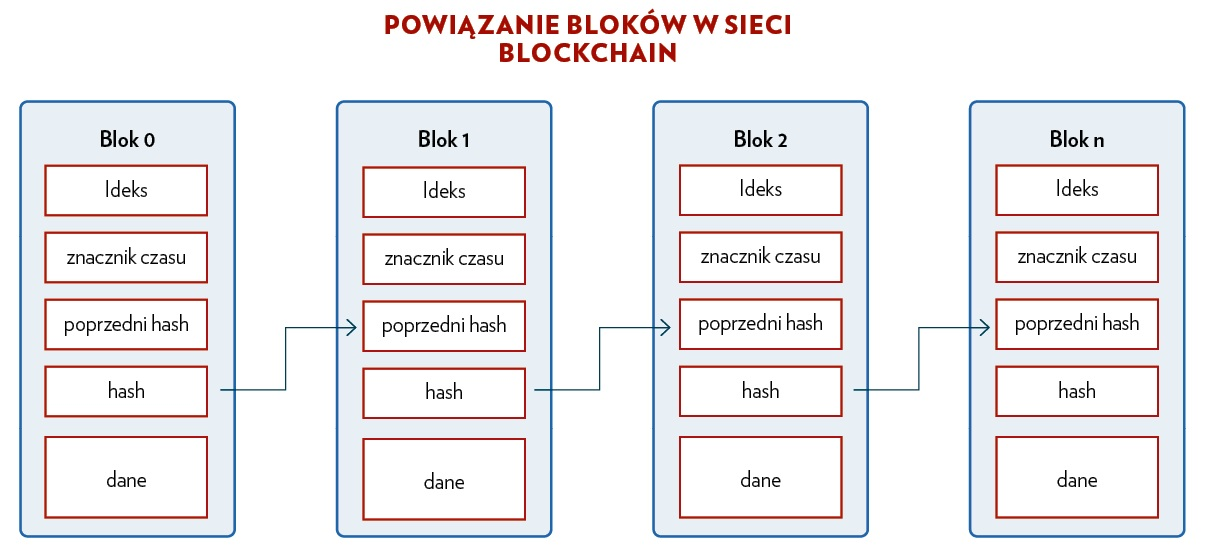
\includegraphics[width=\textwidth]{images/łańcuch_bloków.jpg}
	\caption {Łańcuch bloków.}\label{blocksschain}
\end {figure}

Na rysunku \ref{blocksschain} ukazany jest schemat łańcucha bloków. Jak widać dane przechowywane są w blokach, a bloki połączone są za pomocą wskaźników na \textit{hash} poprzedniego bloku. Taka budowa stanowi zabezpieczenie łańcucha bloków przed modyfikacją lub usunięciem danych. Modyfikacja dowolnego bloku w sieci jest widoczna i łatwa do wykrycia. Wystarczy policzyć od początku \textit{hash} dla każdego bloku i porównać go z polem następnego bloku, które przechowuje poprzedni \textit{hash}.

\subsection{Sieci Peer to Peer}

Zmodyfikowanie łańcucha bloków jest trudne, lecz nie jest niemożliwe. Wymaga wystarczająco dużej mocy obliczeniowej. Dodatkowo zamiast modyfikować łańcuch, można przejąć kontrolę nad urządzeniem, na którym uruchomiony jest łańcuch bloków, co daje możliwość zakłócenia pracy systemu opartego na działaniu łańcucha.

Twórcy Bitcoin'a rozwiązali podane problemy wykorzystując zdecentralizowaną sieć \textit{Peer to Peer}. Sieć \textit{Peer to Peer} składa się z węzłów, które komunikują się ze sobą, bez centralnego serwera. Jeżeli węzły chcą się ze sobą skontaktować, to wysyłają dane bezpośrednio do siebie. Takie rozwiązanie pozwala zwiększyć bezpieczeństwo sieci, ponieważ trudniej jest przejąć kontrolę nad wieloma maszynami tworzącymi całą sieć, niż nad centralnym systemem obsługującym działanie tej sieci. Dodatkowo \textit{Peer to Peer} zapewnia zabezpieczenie danych zgromadzonych w sieci, przed usunięciem, ponieważ każde urządzenie przechowuje swoje egzemplarze danych, które można traktować jako kopie zapasowe. 
Rozproszenie sieci na całym świecie zabezpiecza sieć przed cenzurowaniem, z czego korzysta Bitcoin i inne kryptowaluty.

\textit{Peer to Peer} jest przykładem ciekawego zastosowania architektury klient-serwer. Architektura klient serwer polega na podzieleniu systemu na stronę kliencką, która zajmuje się wysłaniem żądań do serwera, oraz na stronę serwerową, której zadaniem jest odpowiadanie na żądania, przechowywanie danych i operowanie na tych danych. W sieci \textit{Peer to Peer} węzeł pełni rolę zarówno serwera, jak i klienta \cite{p2pbib}. 
Przykładowo węzeł może żądać przesłania danych od innego węzła, a także odpowiedzieć na żądanie innego węzła.

\subsection{Konsensus}

Konsensus w sieci Blockchain to proces, w którym każdy z jej uczestników zgadza się na przeprowadzenie transakcji. Każda aktywność zmieniająca stan przechowywanych danych powinna być zatwierdzona przez uczestników sieci, aby zapewnić bezpieczeństwo i spójność sieci. Konsensus pozwala na wprowadzenie do sieci zestawu reguł, według których działa cała sieć. Takie działanie pozwala na zweryfikowanie zaufanego źródła i wykluczenie wpływu węzłów działających na szkodę sieci \cite{piechk}. W kryptowalutach najczęściej wykorzystywane algorytmy konsensusu to \textit{Proof of Work} i \textit{Proof of Stake}. Istnieje również algorytm \textit{Proof of Authority}, który głownie dotyczy rozwiązań prywatnych sieci Blockchain.

\subsubsection{Proof of Work}

\textit{Proof of Work} to popularny w kryptowalucie Bitcoin algorytm uzyskiwania konsensusu. Algorytm ten wykorzystywany jest podczas tworzenia nowego bloku. Nowy blok wysyłany jest do wszystkich węzłów w sieci, które w celu dodania bloku do swojego łańcucha muszą zostać zatwierdzone. Aby blok został zatwierdzony węzeł musi wykonać pracę, czyli dokonać wkładu mocy obliczeniowej. Moc obliczeniowa wykorzystywana jest do rozwiązania zagadki matematycznej. Praca ta wykonywana jest przez węzeł i jest określana jako \textit{mining} (pol. wydobywanie). Ten węzeł, który jako pierwszy rozwiąże zagadke, otrzyma nagrodę w postaci określonej ilości środków, w kryptowalucie Bitcoin. W typowych rozwiązaniach dla Bitocoin'a poziom trudności dodania nowego bloku jest tak skonstruowany, aby nowe bloki były dodawane, w odstępach około 10 minutowych\cite{pow-bitcoin}.

Takie rozwiązanie premiuje węzły, o większej mocy obliczeniowej. Dlatego w celu utrzymania spójności danych należy przeprowadzać synchronizację węzłów. Synchronizacja przebiega nastepująco: każdy węzeł rozsyła do całej sieci swój łańcuch, węzły porównują długość swojego łańcucha z nadesłanym łańcuchem i w węźle zapisywany jest dłuższy łańcuch.

\textit{Proof of work} to rozwiązanie towarzyszące architekturze Blockchain, od momentu jej powstania. Bitcoin poza dokonywaniem transakcji, pozwala na zarabianie poprzez tworzenie tzw. węzłów górniczych. Węzeł górniczy zajmuje się realizacją algorytmu \textit{Proof of Work}, co oznacza rozwiązywanie zagadki matematycznej. Fizycznie jest to urządzenie, ze specjalistycznymi podzespołami i oprogramowaniem, które pozwala na uzyskanie wysokiej efektywności w wydobywaniu Bitcoin'a \cite{nodes}. Głównym problemem tego rozwiązania jest zużycie energii elektrycznej. W roku 2017 zużycie energii elektrycznej, przez wydobywanie Bitcoin'a było większe, niż w 159 krajach na świecie \cite{elctricity-bitcoin}. W roku 2019 naukowcy z \textit{University of Cambridge} stworzyli specjalny indeks \textit{CBECI} (Cambridge Bitcoin Electricity Consumption Index), ukazujący dane dotyczące zużycia energii elektrycznej, przez Bitcoin'a \cite{CBECI}.

W tym algorytmie czynnik wkładu fizycznych zasobów, jest głównym motywatorem do uczciwego postępowania. Jednakże głownym czynnikiem sprawiającym, że ten algorytm działa jest pewność, że ponad 50\% uczestników sieci działa uczciwie. Ogrom inwestowanych zasobów wpływa na bezpieczeństwo sieci. Duża zdecentralizowana sieć Blockchain dysponuje ogromną mocą obliczeniową, na jej moc składa się moc wszystkich węzłów w sieci. Węzły różnią się mocą obliczeniową, natomiast decentralizacja sieci sprawia, że żaden z węzłów nie może przejąć kontroli nad całą siecią. Im większa decentralizacja tym bardziej zmniejsza się wpływ pojedynczego węzła na całą sieć. Co innego, gdy do sieci dołączona zostanie grupa węzłów, które będą stanowiły 51\% mocy obliczeniowej sieci oraz będą ze sobą współpracowały, działając na szkodę sieci. Taki scenariusz nazywany jest atakiem 51\%. Dysponując 51\% mocy obliczeniowej sieci, można bez wiedzy uczciwych uczestników, w szybszy sposób dodawać nowe bloki, co prowadzi do przejęcia obsługi dodawania zawartości, przez szkodliwych uczestników sieci\cite{atack51}.

W przypadku dużych kryptowalut atak 51\% jest bardzo rzadkim zjawiskiem, gdyż jest on bardzo drogi. Atak ten może być opłacalny jedynie wtedy, gdy atakujący chce zdestabilizować sieć. W przypadku Bitcoin'a destabilizacja sieci nie ma większego sensu, ponieważ dysponując taką mocą obliczeniową można uzyskać ogromne przychody z kopania Bitcoin'a, dodatkowo uzyskanie takiej mocy obliczeniowej w rozrastających się sieciach Blockchain dla Bitcoin'u jest na tyle drogie, że w teorii jest uznawane za nieosiągalne. Z tego powodu, w przypadku sieci Blockchain, bardzo ważne jest zadbanie o jak największe rozproszenie węzłów w sieci \textit{Peer to Peer}\cite{abpow}.

\subsubsection{Proof of Stake}

\textit{Proof of Stake} to kolejny algorytm używany do osiągania konsensusu w sieciach Blockchain. Jego największą zaletą jest rozwiązanie problemu wykorzystania ogromnych ilości zasobów energii elektrycznej, przez algorytm \textit{Proof of Work}.

Działanie algorytmu \textit{Proof of Stake} polega na wybieraniu spośród dostępnych węzłów sieci Blockchain walidatora. Walidator to węzeł, którego zadaniem jest weryfikacja poprawności bloku dołączanego do łańcucha. Wybór walidatora może się odbywać na różne sposoby, od całkowicie losowego wyboru, po wybór z uwzględnieniem czynników takich jak np. wiek stawki węzła, wysokość stawki. Stawka to zablokowane na koncie danego węzła jednostki waluty (kryptowaluty). Stawka jest wymagana, aby węzeł mógł uczestniczyć w losowaniu.

W przypadku algorytmu \textit{Proof of Stake} głównym motywatorem uczciwego uczestnictwa w sieci jest możliwość utracenia części stawki. W przypadku wykrycia przez sieć nieprawidłowości w bloku dodanym przez konkretny węzeł, traci on określoną część stawki.

\textit{Proof of Stake} jest o wiele bardziej ekologiczny, jeśli chodzi o zużycie energii elektrycznej, niż \textit{Proof of Work}. W \textit{Proof of Stake} głównym czynnikiem determinującym moc sieci jest zgromadzony w niej wkład finansowy w postaci stawek. W przypadku tego algorytmu również występuje problem ataku 51\%, jednakże tym razem atakujący musi dysponować odpowiednią ilością środków płatniczych, a dokładnie musi włożyć 51\% ogólnej stawki, co w przypadku Bitcoin'a jest mało prawdopodobne \cite{abpos}.

\subsubsection{Proof of Authority}
\textit{Proof of Authority} to rozwiązanie skłaniające się ku mniej zdecentralizowanym systemom, które są tworzone na prywatne potrzeby i wymagają dużej przepustowości. \textit{Proof of Authority} jest w swoim działaniu nieco zbliżony do \textit{Proof of Stake}. Zamiast stawki podanej w jednostkach odpowiedniej waluty, w \textit{Proof of Authority} używana jest reputacja walidatora. Prowadzi to do skonstruowania sieci, w której uczestniczą tylko zaufani walidatorzy. Uzyskanie statusu walidatora wiąże się z dużym nakładem pracy, w celu spełnienia kryteriów i uzyskania odpowiednio wysokiej reputacji. Podczas projektowania takiego systemu należy zwrócić szczególna uwagę, na stworzenie kryteriów o wysokiej trudności do spełnienia, aby wykluczyć węzły o szkodliwym działaniu.

Trudność uzyskania statusu walidatora bardzo mocno wpływa na stopień zdecentralizowania. Decentralizacja porównywalna z rozwiązaniem \textit{Proof of Stake} jest niemożliwa do osiągnięcia.
Niski stopień decentralizacji wymaga pełnego zaufania do walidatorów, co może stanowić słaby punkt systemu, gdy zaufany walidator zostanie przekupiony i dokona szkodliwej manipulacji na zawartości systemu.

Algorytm \textit{Proof of Authority} świetnie sprawdza się w prywatnych sieciach Blockchain, gdy ważna jest wysoka przepustowość łącza. Jednakże należy pamiętać o odpowiednim doborze walidatorów\cite{abpoa}.

\subsection{Funkcja skrótu}

Funkcje skrótu w systemach informatycznych pełnią rolę zabezpieczenia integralności danych. Zabezpieczenie danych polega na wykryciu ich modyfikacji. Matematyczna definicja funkcji skrótu \textit{h} to odwzorowanie wiadomości \textit{m} o dowolnej, skończonej długości, w ciąg bitów o określonej, stałej długości \textit{n} \cite{hash}:

\begin{equation}
h:\left \{0, 1\right \}^{*}\rightarrow \left \{0, 1\right \}^{n}, gdzie: \left \{0, 1\right \}^{*}=\bigcup_{i\in  N}\left \{0, 1\right \}^{i}, N = \left \{0, 1, ...\right \}, n \in N
\end{equation}

Funkcja skrótu cechuje się wysoką podatnością na zmiany. Zmiana jednego bitu w danych wejściowych powoduje otrzymanie zupełnie innych wyników. \newline
Przykładowo dla ciągu znaków \textit{hash0}, dla funkcji skrótu \textit{SHA256} wynikiem jest ciąg znaków
\newline \textit{6ac73742db534bebccc9af1453c5637ee5bb5d7c9628ec2f26cf9777c89e96d8}. Natomiast zmieniając ciąg znaków na \textit{hash1}, otrzymanym wynikiem jest \newline \textit{af316ecb91a8ee7ae99210702b2d4758f30cdde3bf61e3d8e787d74681f90a6}. Przykład obrazuje jak na wynikowy ciąg znaków wpływa zmiana jednego symbolu na wejściu.

Głównymi cechami funkcji skrótu są:
\begin{itemize}
	\item Nieodwracalność - na podstawie otrzymanego wyniku nie można bezpośrednio odtworzyć danych.
	\item Bezkolizyjność - nie istnieją dwa różne ciągi znaków, które dają ten sam wynik.
\end{itemize}

Znalezienie danych wejściowych dla funkcji skrótu jest zadaniem wymagającym dużego nakładu mocy obliczeniowej. Dane można uzyskać losując wejściowy ciąg znaków i \textit{hash'ując} go, a następnie porównując otrzymany \textit{hash} z \textit{hash'em}, który ma być rozszyfrowany. Jest to tak zwany atak brutalny (ang. brute force).

Popularnym zastosowaniem funkcji skrótu jest podpis cyfrowy. Podpis cyfrowy to zaszyfrowany \textit{hash}, wygenerowany na podstawie danych potrzebnych do podpisu. Główną zaletą wykorzystania \textit{hash'owania} w podpisie cyfrowym jest szybkość. \textit{Hash'owanie} wiadomości jest szybsze od szyfrowania, a zaszyfrować wystarczy sam ciąg znaków o stosunkowo małej długości, w porównaniu do tekstu wiadomości.

Funkcje skrótu można spotkać w bazach danych. Hasła są przykładem informacji, które w bazie danych są przechowywane w postaci funkcji skrótu. Takie rozwiązanie zabezpiecza hasła, w przypadku wycieku danych. \cite{hash}

\subsection{Smart kontrakty}

Wraz z powstaniem kryptowaluty Ethereum do architektury Blockchain została dodana nowa funkcja. Dodano tak zwane \textit{smart} kontrakty, które pozwalają na zaprogramowanie i uruchomienie kodu w sieci Blockchain. Takie programy można stosować, w celu kontrolowania sieci poprzez zdefiniowanie zestawu reguł dla sieci. Zdefiniowanie zestawu reguł pozwala na zwiększenie zaufania w sieci, a także automatyzację niektórych procesów.

\textit{Smart} kontrakty pozwalają na tworzenie aplikacji, których podstawą jest Blockchain. Przykładem środowiska pozwalającego na tworzenie takich programów jest język Solidity, który został stworzony dla sieci Ethereum\cite{smart-contract}. 

\newpage

\section{Technologia Blockchain na rynku}

Technologia Blockchain jest wykorzystywana w wielu dziedzinach życia, a jej głównym zadaniem jest zapewnienie bezpieczeństwa danychj. 

\subsection{Kryptowaluty}

Kryptowaluta to cyfrowy środek płatniczy. W przeciwieństwie do tradycyjnych walut, kryptowaluty nie są kontrolowane przez bank centralny. Środki płatnicze w kryptowalucie znajdują się w rozproszonej, po całym świecie sieci. Każda transakcja w tym środowisku jest zapisywana we współdzielonym rejestrze. Rejestr pozwala na ustalenie ile środków w danej kryptowalucie jest na koncie danego uczestnika sieci. Podstawą działania kryptowalut jest Blockchain. To Blockchain odpowiada za tworzenie rejestru transakcji, zabezpieczenie danych przed modyfikacją, współdzielenie danych i uzyskanie konsensusu. Przykładem takich kryptowalut są Bitcoin i Ethereum. \cite{bitcoin}

\subsection{Finanse}

Dynamiczny rozwój technologii zapoczątkował rozwój innych branż, w tym sektora finansów. Powstała osobna gałąź tego sektora o nazwie FinTech. FinTech zajmuje się opracowywaniem i wdrażaniem nowych technologii do systemów finansowych na całym świecie. Korzyści płynące z unowocześnienia sektora finansów mogą skupiają się głównie na zwiększeniu szybkości transakcji przez brak pośredników, zmniejszeniu kosztów przepływu transakcji i zwiększenie bezpieczeństwa. FinTech zajmuje się między innymi szukaniem zastosowań dla technologii Blockchain. Jako przykład rozwijania technologii blockchain przez FinTech może posłużyć przykład trwałego nośnika wdrożonego przez PKO Bank Polski. Trwały nośnik pozwala na dostarczanie klientom banku prywatnych dokumentów w formie cyfrowej \cite{PKO}. Twórcy tego rozwiązania zastosowali również mechanizm Smart Kontraktów. Smart Kontrakty są wykorzystywane do zautomatyzowania procesu egzekwowania umów ubezpieczeniowych\cite{PKO-SMART}. Pozwala to na zmniejszenie uczestnictwa osób trzecich i redukcję kosztów.

\subsection{Internet of Things}

Internet of Things to technologia pozwalająca na łączenie ze sobą wielu urządzeń. Tak skonstruowane sieci znajdują swoje przeznaczenie w systemach czasu rzeczywistego w przemyśle, bądź w inteligentnym domu. IoT wykorzystuje serwery internetowe, do przechowywania i pobierania danych. Blockchain w usługach IoT pomaga zabezpieczyć serwery z danymi, poprzez ich decentralizację. \cite{abiot}

\newpage

\chapter{E-voting}
W tym rozdziale znajduje się przegląd istniejących rozwiązań wyborów \textit{on-line}, które są dostępne na rynku. System estoński jest przykładem wykorzystania wyborów \textit{on-line} przez struktury państwowe, a E-voting w Walnych Zgromadzeniach jest przykładem rozwiązania stworzonego na prywatne potrzeby.

\section{System estoński}
Przykładem regularnego wykorzystania e-votingu jest Estonia. Estonia jest krajem, który pierwszy udostępnił możliwość głosowania elektronicznego w wyborach lokalnych, na szczeblu krajowym. W pierwszych wyborach wzięło udział około 1\% wyborców. Od roku 2005 w Estonii postępował rozwój systemów e-votingu. Wraz z następnymi wyborami zwiększała się liczba uczestników. W roku 2019 liczba wyborców, którzy skorzystali z e-votingu wyniosła 43,8\% wyborców.

Na system e-votingu w Estonii składa się kilka mniejszych rozwiązań:
\begin{itemize}

\item identyfikacja za pomocą karty e-obywatela lub profilu e-obywatela w telefonie,

\item architektura rozwiązania pozwala na wysłanie wielu głosów, a głosem wiążącym jest zawsze głos finalny,

\item serwery wykorzystywane podczas głosowania są pod szczególną ochroną i nie można uzyskać do nich dostępu z bezpośrednio z internetu (zabezpieczenie firewall'em),

\item wykorzystywanie prywatnych kluczy i narzędzi kryptograficznych w celu zabezpieczenia dostępu do danych. Wykorzystywanie standardu SSL (ang. Secure Sockets Layer).
\end{itemize}

\subsection{Przegląd rozwiązania}
Rysunek \ref{estmodules} przedstawia moduły systemu estońskiego, które wchodzą w skład przebiegu całego procesu wyborów. Przebieg całego procesu wyborczego w Estonii można podzielić na kilka etapów:
\begin{itemize}
\item ogłoszenie wyborów,
\item zarejestrowanie kandydatów,
\item przygotowanie list wyborczych,
\item głosowanie,
\item liczenie głosów,
\item ogłoszenie wyników.
\end{itemize}

Wsparcie e-votingu (w Estonii określanego i-votingiem) obejmuje ostatnie trzy etapy procesu wyborczego.

\begin{figure}[h]
	\centering
	\includegraphics[width=\textwidth]{images/Dziedzina systemu estońskiego}
	\caption{Moduły systemu i-votingu. \cite{estonian:voting}}\label{estmodules}
\end {figure}
\newpage

W skład systemu głosowania wchodzą bazy danych (rys. \ref{estmodules}) przechowujące:
\begin{itemize}
\item listę osób uprawnionych do głosowania,
\item listę okręgów wyborczych,
\item listę kandydatów lub opcji wyborczych,
\item listę e-wyborców (na rys. \ref{estmodules} \textit{i-voters}).
\end{itemize}

Dostarczenie odpowiednich danych do systemu pozwala na walidację wyborcy, zgłoszenie przez
niego głosu oraz zapisanie wyborcy, w bazie danych odpowiedzialnej za przechowanie listy e-wyborców. W skład logiki systemu wchodzą mechanizmy generujące wyniki. Wyniki e-votingu są scalane z wynikami wyborów tradycyjnych, przy czym scalanie nie pozwala na podwójne zliczanie głosu oddanego tradycyjnie i elektronicznie.

\begin{figure}[h]
	\centering
	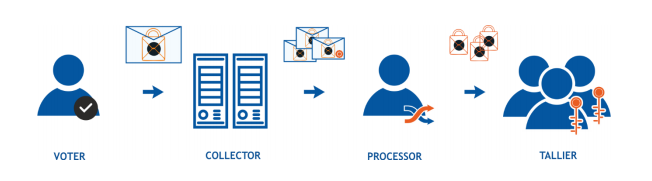
\includegraphics[width=\textwidth]{images/Główne częsci systemu estońskiego.png}
	\caption{Proces wyborczy. \cite{estonian:voting}}\label{estprocess}
\end {figure}

Rysunek \ref{estprocess} przedstawia proces wyborczy. W tym procesie można wyróżnić nastepujących aktorów:
\begin{itemize}
\item \textit{voter} (wyborca) - za pośrednictwem aplikacji klienckiej (która w systemie estońskim jest aplikacją desktopową pobieraną przed wyborami) szyfruje i potwierdza swoim podpisem elektronicznym głos, który następnie wysyłany jest do zbieracza głosów,
\item \textit{collector} (zbieracz głosów) - to aplikacja serwerowa wyposażona w logikę pozwalającą na utworzenie głosu. Aplikacja waliduje dane wprowadzone przez wyborcę i elektronicznie podpisuje dane, które następnie przesyła do procesora,
\item \textit{processor} (procesor głosów) - zajmuje się przetwarzaniem głosów. Sprawdza poprawność danych otrzymanych z zbieracza głosów, wraz z podpisem elektronicznym. Usuwa głosy, które się powtarzają, zarówno głosy oddane elektronicznie, jak i te oddane w lokalach wyborczych. Sortuje głosy według okręgów wyborczych i usuwa z nich podpis elektroniczny, w celu anonimizacji głosu. Tak przetworzone głosy są mieszane według odpowiedniego algorytmu i wysyłane do Licznika,
\item \textit{tallier} (licznik głosów) - rolą licznika jest odebranie głosu od procesora, otwarcie go i dodanie przyporządkowanie do odpowiedniego wyniku.
\end{itemize}

Estoński system e-votingu jest spójny i dobrze zabezpieczony. Dlatego jest on wykorzystywany w ważnych wyborach krajowych. Rozwiązanie jest stale udoskonalane, aby mogło dotrzymać kroku rozwojowi technologii.\cite{estonian:voting}

\section{Evoting w Walnych Zgromadzeniach}

Krajowy Depozyt Papierów Wartościowych (KDPW) to instytucja finansowa, której zadaniem jest nadzorowanie i prowadzenie rejestracji obrotu instrumentami finansowymi w Polsce. KDPW pełni również rolę depozytu papierów wartościowych. KDPW jest spółką akcyjną, której współwłaścicielami są akcjonariusze - państwo (Skarb Państwa) i państwowe spółki finansowe (Giełda Papierów Wartościowych, Narodowy Bank Polski).

Walne Zgromadzenie to organ mający najwyższe uprawnienia w spółce akcyjnej. Walne Zgromadzenie pozwala akcjonariuszom na zarządzanie spółką. Podczas Walnego Zgromadzenia podejmuje się uchwały dotyczące spółki akcyjnej.

Krajowy Depozyt Papierów Wartościowych udostępnia swoim akcjonariuszom aplikacje eVoting oraz Walne Zgromadzenia, które przenoszą proces przeprowadzania Walnego Zgromadzenia do internetu. Zgodnie z art. 402 Kodeksu Spółek Handlowych \cite{sp-han}, Walne Zgromadzenie zwoływane jest przez ogłoszenie go, co najmniej trzy tygodnie przed zaplanowanym terminem. W celu zwołania Walnego Zgromadzenia w aplikacji Evoting i Walne Zgromadzenia należy zarejestrować walne zgromadzenie. KDPW przesyła ogłoszenie, o Walnym Zgromadzeniu do jego uczestników. Wymiana informacji odbywa się drogą elektroniczną.
Uczestnicy tworzą listę osób uprawnionych do udziału w Walnym Zgromadzeniu, która jest przesyłana do KDPW. KDPW generuje wykaz osób uprawnionych do uczestnictwa w Walnym Zgromadzeniu, a następnie dostarcza informacje o uczestnictwie w Walnym Zgromadzeniu indywidualnie, dla każdego uczestnika. Każdy uczestnik otrzymuje również kod autoryzacyjny, który wykorzystywany jest do potwierdzenia tożsamości uczestnika, w celu przyznania uprawnień do uczestnictwa w walnym zgromadzeniu. Przyznanie uprawnień jest równoznaczne z potwierdzeniem obecności na walnym zgromadzeniu i udostępnieniu uczestnikowi interfejsu do głosowania \cite{eVoting-dzialanie}.

Za zapewnienie nieodwracalności wykonanych akcji i ogólnego bezpieczeństwa danych, w aplikacjach eVoting i Walne Zgromadzenia jest odpowiedzialny Blockchain.

\chapter{Wymagania systemu i wykorzystane narzędzia}
W tym rozdziale sformułowano i omówiono wymagania funkcjonalne i niefunkcjonalne. Dodatkowo przedstawiono przypadki użycia i aktorów systemu. Na koniec opisane zostały technologie i narzędzia wykorzystane podczas tworzenia systemu.

\section {Wymagania niefunkcjonalne}

Wymagania niefunkcjonalne definiują jakość usług dostarczanych przez system. W systemie e-votingu ważnymi elementami są bezpieczeństwo i czytelność procedury głosowania. Dlatego w celu uściślenia oczekiwań jakościowych systemu sformułowano następujące wymagania niefunkcjonalne:

\begin{itemize}
	\item dane logowania użytkownika są zabezpieczone,
	\item dane logowania administratora są zabezpieczone,
	\item przechowywane głosy są zabezpieczone przed modyfikacją,
	\item przejrzyste treści na stronie wyborcy,
	\item czytelna i łatwa w obsłudze procedura wyborcza na stronie wyborcy,
	\item przejrzyste treści na stronie administratora wyborów,
	\item czytelna i łatwa w obsłudze konfiguracja wyborów,
	\item aplikacje internetowe wyborcy i administratora działają na najpopularniejszych przeglądarkach internetowych.
	\item czas liczenia głosów jest zdeterminowany.
\end{itemize}

\section {Wymagania funkcjonalne}

W tej sekcji umieszczono wszystkie funkcjonalności i części systemu. Do głównych części systemu należą: aplikacja internetowa wyborcy, aplikacja internetowa administratora wyborów,
serwis udostępniający REST API i serwery sieci Blockchain. Do wymagań funkcjonalnych systemu należą:

\begin{itemize}
	\item hasła przechowywane w bazie danych są szyfrowane za pomocą funkcji skrótu \textit{SHA256},
	\item dostęp do zasobów wyborcy i administratora odbywa się poprzez dwie różne aplikacje internetowe,
	\item komunikacja pomiędzy aplikacjami przeglądarkowymi, a API odbywa się z wykorzystaniem konwencji REST API,
	\item dostęp do punktów końcowych API (tzw. endpoint'ów) jest zabezpieczony za pomocą JWT (Json Web Token) oraz uwierzytelnienia na podstawie roli (Role Based Authentication),
	\item dostęp do zasobów posiadają tylko zalogowani użytkownicy,
	\item za bezpieczne przechowywanie głosów odpowiada sieć Blockchain,
	\item każdy węzeł sieci Blockchain to indywidualny program posiadający własną konfigurację,
	\item dla każdych wyborów konfigurowana jest indywidualna sieć Blockchain,
	\item dostęp do sieci Blockchain uzyskiwany jest za pomocą serwisu,
	\item komunikacja pomiędzy serwisem, a siecią Blockchain odbywa się z udziałem jednego węzła, który odbiera informacje i rozsyła po całej sieci,
	\item konsensus w sieci może zostać uzyskany z wykorzystaniem algorytmu \textit{Proof of Work} lub algorytmu opratego o \textit{Proof of Authority}.
\end{itemize}

\newpage

\section{Diagramy przypadków użycia}

W systemie można wyróżnić dwóch aktorów. W tym podrozdziale zostały przedstawione i omówione diagramy przypadków użycia dla tych aktorów.

\begin{figure}[h]
	\centering
	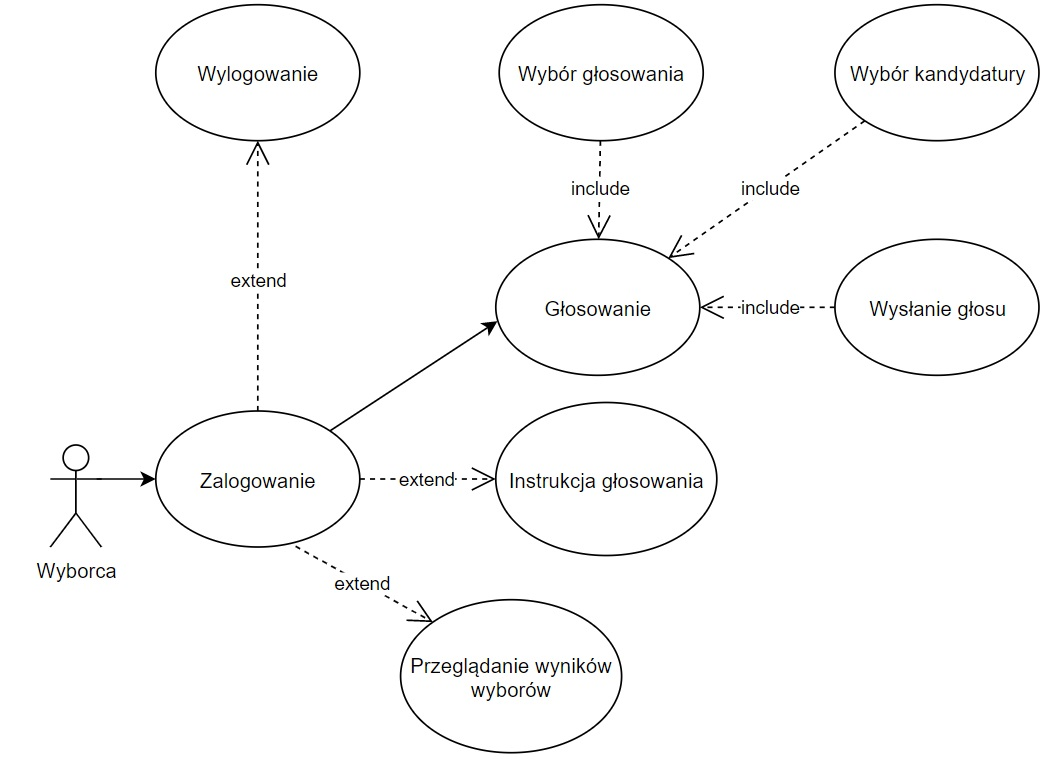
\includegraphics[width=\textwidth]{images/user_use_case.jpg}
	\caption{Diagram przypadków użycia wyborcy.}\label{user-use}
\end {figure}

Pierwszym z wyszczególnionych aktorów jest użytkownik aplikacji, czyli wyborca. Przewidziane akcje dostępne dla wyborcy to zalogowanie, wylogowanie, dostęp do instrukcji głosowania, głosowanie i odbiór wyników wyborów. Rysunek \ref{user-use} przedstawia diagram przypadków użycia dla wyborcy.

Drugim aktorem występującym w systemie jest administrator wyborów. Do zadań administratora należą: 

\begin{itemize}
	\item tworzenie wyborów - konfiguracja składników wyborów,
	\item modyfikacja wyborów - nadzorowanie procesu wyborczego,
	\item dodawanie wyborców do bazy danych - zarządzanie kontami wyborców,
	\item ogłoszenie wyników wyborów.
\end{itemize}

Dodatkowo administrator posiada swoje konto w systemie. Aby mógł korzystać z przydzielonych mu zasobów musi się zalogować. Rysunek \ref{admin-use} przedstawia diagram przypadków użycia dla administratora wyborów.

\begin{figure}[h]
	\centering
	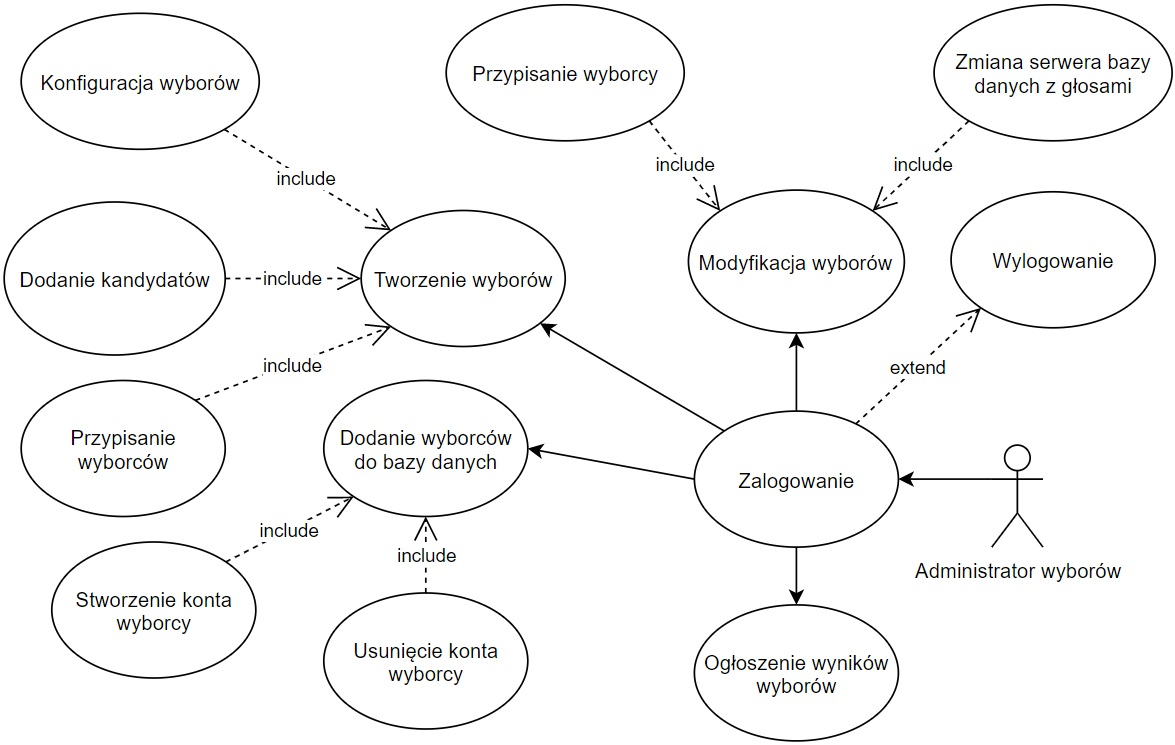
\includegraphics[width=\textwidth]{images/admin_use_case.jpg}
	\caption{Diagram przypadków użycia administratora.}\label{admin-use}
\end {figure}

\newpage
\section {Wykorzystane narzędzia i technologie}

System e-votingu składa się z wielu modułów, których stworzenie obejmuje różne dziedziny programowania. W systemie są elementy odpowiedzialne za interfejs użytkownika, aplikację serwerową i bazę danych. Każdy z tych rodzajów oprogramowania wymaga innego podejścia. Są to popularne dziedziny programowania, dlatego znalezienie rozwiązań nie stanowi problemu. W tej sekcji przedstawiono wykorzystane narzędzia i technologie.

\subsection{Interfejs użytkownika}

W celu stworzenia rozbudowanego interfejsu użytkownika wykorzystano bibliotekę javascript-ową - ReactJs. React pozwala na tworzenie aplikacji internetowych z wykorzystaniem języków JavaScript, HTML i CSS. Takie podejście do tworzenia aplikacji określane jest jako SPA (Single Page Application), taka aplikacja posiada jeden plik \textit{.html}, którego zawartość jest dynamicznie generowana w trakcie działania aplikacji. Podejście typu SPA pozwala na zredukowanie liczby zasobów potrzebnych do generowania strony, poprzez wykorzystanie tylko jednego pliku \textit{.html}. Strona typu SPA działa płynnie, ponieważ nie wymaga ona ładowania szablonów z plików \textit{.html}. Ważną cechą ReactJs jest podejście do tworzenia interfejsu użytkownika, jak do grupy komponentów. Komponent może być dowolnym elementem interfejsu, od paska nawigacji do przycisku. Każdy komponent posiada swój stan, czyli zestaw zmiennych kontrolujących jego funkcjonalności. Takie podejście pozwala na tworzenie uniwersalnych i konfigurowalnych komponentów, które można wykorzystywać w wielu miejscach aplikacji.

Biblioteka ReactJs to bardzo rozbudowane narzędzie, które dzięki swojej popularności posiada wiele dodatkowych rozwiązań współpracujących z całym środowiskiem ReactJs. Przykładem takiego dodatku jest biblioteka Redux, która pozwala na zarządzanie stanem aplikacji. Redux pozwala przenieść stan z komponentu do osobnego kontekstu. Takie rozwiązanie pozwala na umieszczenie tych części stanu aplikacji, które odnoszą się do różnych komponentów w jednym kontenerze. Stan aplikacji jest dostępny globalnie, a nie tylko dla komponentów potomnych. Przykładowo stan informujący o zalogowaniu do aplikacji powinien być dostępny dla całej aplikacji. Przeniesienie tego stanu do osobnego kontekstu pozwala na zdefiniowanie go w jednym miejscu i dostarczenie do odpowiednich komponentów. W projekcie wykorzystano opartą na Redux, bibliotekę Redux-Toolkit. Głównym argumentem za wykorzystaniem Redux-Toolkit jest mniejsza objętość kodu, która powstaje do uzyskania rozwiązania.

Podstawowym narzędziem odpowiedzialnym za wygląd interfejsu aplikacji internetowej są kaskadowe arkusze stylów, czyli popularny CSS (Cascade Style Sheets). Język CSS jest jedynym językiem odpowiedzialnym za określenie wyglądu strony internetowej, który jest rozumiany przez przeglądarkę. Jednakże istnieją rozwiązania, które pozwalają na wprowadzenie nowej składni z zachowaniem kompatybilności z danym środowiskiem uruchomieniowym (w tym przypadku z przeglądarką). Są to tzw. \textit{preprocesory}. Preprocesor pozwala na przetworzenie danego kodu źródłowego, na określony kod wyjściowy. Przykładem preprocesora języka CSS, który został wykorzystany w projekcie jest SASS(Syntactically Awesome Style Sheets). SASS dostarcza funkcjonalności, które nie są dostępne w języku CSS. Przykładowo SASS pozwala na zagnieżdżanie instrukcji, deklarowanie i wywoływanie zmiennych oraz tzw. \textit{mixin'y}, które pozwalają na zadeklarowanie powtarzających się fragmentów kodu w jednym miejscu i ich wywoływanie bez konieczności przepisywania kodu. Sass pozwala na lepsze wykorzystanie dobrych praktyk programowania, takich jak uniknięcie powtarzania kodu.

Jak już wspomniano w tej sekcji ReactJs jest popularną biblioteką, co przekłada się na dużą liczbę rozszerzeń i dodatków. Dodatki obejmują również stylowanie aplikacji. W projekcie została wykorzystana biblioteka Material-Ui, która dostarcza gotowe zestawy komponentów i narzędzia do ich stylowania. Zaletą tego rozwiązania jest wykorzystywanie komponentów, które stworzono z użyciem dobrych praktyk tworzenia interfejsu użytkownika.

Aplikacje internetowe często wymagają komunikacji z zewnętrznym serwerem, w celu pobrania lub wysłania odpowiednich zasobów. Istnieje wiele rozwiązań, które pozwalają na wysyłanie żądań w standardzie HTTP (Hypertext Transfer Protocol). W projekcie wykorzystano javascript-ową bibliotekę Axios. Biblioteka dostarcza wiele mechanizmów do wysyłania żądań HTTP, a jej wielką zaletą jest łatwość obsługi.

JavaScript to język programowania, który świetnie sprawdza się w środowisku aplikacji przeglądarkowych. Język umożliwia wieloaspektowe podejście do programowania. Można pisać programy w sposób deklaratywny lub obiektowy. JavaScript spełnia standardy nowoczesnych języków programowania, o czym świadczyć może ogromna popularność tego języka. Jednakże niektóre właściwości tego języka mogą utrudniać tworzenie oprogramowania. Przykładem jest dynamiczne typowanie.W JavaScript każda zmienna nie ma przypisanego typu na stałe. Takie rozwiązanie ma swoje wady i zalety, jednak są przypadki, w których programista powinien mieć wybór, kiedy użyć zmiennej typowanej dynamicznie, a kiedy nie. Rozwiązaniem tego problemu jest język Typescript. Typescript jest nadzbiorem JavaScript co oznacza, że dostarcza on wszystkie funkcje JavaScript'u i jednocześnie rozszerza go o nowe. W Typescript można deklarować zmienne z określonym typem, a także używać typu \textit{any}. Typ \textit{any} określa zmienne, które mogą być typowane dynamicznie. Język Typescript dostarcza również możliwość definiowania własnych typów. W projekcie, w celu uniknięcia problemów związanych z dynamicznym typowaniem wykorzystano język Typescript.

\subsection{Serwer}
Za stronę serwerową aplikacji odpowiada silnik NodeJs. NodeJs pozwala na tworzenie aplikacji w JavaScript, poza środowiskiem przeglądarkowym. Silnik stanowi również rozbudowane narzędzie pozwalające na tworzenie REST API. Zaletą NodeJs jest ogromna popularność, co jest zauważalne podczas szukania rozwiązań w internecie na napotkane problemy. Popularność silnika przekłada się również na jego bogatą dokumentację i dodatkowe biblioteki, które usprawniają proces tworzenia oprogramowania.

ExpressJs to biblioteka działająca na silniku NodeJs, która została wykorzystana w projekcie do tworzenia REST API i węzłów sieci Blockchain. ExpressJs dostarcza podstawowe narzędzia do tworzenia REST API, takie jak tworzenie punktów końcowych serwera, które pozwalają na obsługiwanie żądań HTTP. Zaletą biblioteki ExpressJs jest kompatybilność z wieloma innymi bibliotekami przeznaczonymi dla silnika NodeJs.

Prisma to jedna z bibliotek NodeJs, które są odpowiedzialne za obsługę bazy danych. Prisma dostarcza mechanizm ORM (Object Relational Mapping), czyli możliwość odwzorowania relacyjnej bazy danych, na obiekty danego języka programowania. Prisma generuje moduły odpowiedzialne za obsługę bazy danych i dostarcza je programiście. Takie rozwiązanie pozwala na utrzymanie całości aplikacji w jednym języku programowania, ponieważ nie wymaga korzystania z języka SQL (Structured Query Language). Wszystkie moduły obsługi bazy danych tworzone są automatycznie, dlatego Prisma pozwala oddzielić implementację bazy danych, od innych funkcjonalności aplikacji.

\subsection {Baza danych}

Wykorzystana baza danych działa na silniku SQLite. Baza danych znajduje się w pliku i jest umieszczona na serwerze wraz z REST API. SQLite to szybki, mały i łatwy w konfiguracji silnik baz danych. Jest to świetny silnik do prototypowania i tworzenia małych, a zarazem przenośnych baz danych.

Silnik SQLite można obsługiwać z poziomu konsoli lub za pomocą specjalnej aplikacji, która dostarcza interfejs graficzny prezentujący zawartość bazy danych. W projekcie wykorzystano aplikację SQLiteStudio, która pozwala na połączenie się z bazą danych, w celu zarządzania nią. SQLiteStudio pozwala na tworzenie tabel, dodawanie zawartości, usuwanie danych i przeszukiwanie bazy danych. Aplikacja pozwala również na pisanie własnych zapytań w języku SQL. Tego rodzaju aplikacje są przydatne podczas tworzenie tabel w bazie danych i testowania aplikacji.

\subsection{Testowanie}

Testowanie strony serwerowej systemu odbywało się przez aplikację Postman, która pozwala na wysyłanie żądań HTTP. W aplikacji można skonfigurować żądanie HTTP, tak aby zasymulować odpowiednie scenariusze żądania. Pozwala to przetestować działanie wszystkich funkcjonalności API.

Testowanie aplikacji w środowisku lokalnym pozwala odpowiedzieć na pytanie, czy całość komponentów działa w kontrolowanym środowisku. Natomiast przeniesienie aplikacji do sieci pozwala na przetestowanie wydajności aplikacji. W projekcie, w celu udostępnienia aplikacji w internecie wykorzystano serwisy Netlify oraz Heroku. Netlify pozwala na udostępnienie aplikacji internetowej, pod adresem generowanym przez serwis. Heroku zajmuje się uruchomieniem aplikacji serwerowej, która również dostępna jest w sieci pod odpowiednim adresem.

\subsection{Metodyka pracy}
 
Do prowadzenia projektu wykorzystano repozytorium kontroli wersji GitHub. GitHub to narzędzie, które pozwala przechowywać kod źródłowy aplikacji, a także zapewnia jego archiwizację i wersjonowanie. Do przydatnych funkcji należy również tworzenie rozgałęzień na różnych etapach tworzenia aplikacji. Pozwala to na oddzielenie poszczególnych funkcji na odrębne gałęzie projektu. Takie podejście pozwala na uporządkowanie pracy nad projektem i większą przejrzystość w procesie rozwoju modułów.
 
GitHub pozwala również na synchronizację ze wspomnianymi Heroku i Netlify, co pozwala na automatyzację procesu umieszczania nowych wersji aplikacji w środowisku internetowym. Wraz z umieszczeniem nowej wersji aplikacji w repozytorium, serwisy otrzymują kod źródłowy za pośrednictwem GitHuba, a następnie budują i uruchamiają aplikację.
 
%%%%%%%%%%%%%%%%%%%%%%%%%%%%%%%% Specyfikacja zewnętrzna %%%%%%%%%%%%%%%%%%%%

\chapter{Specyfikacja zewnętrzna}
Ten rozdział zawiera szczegółowy opis funkcjonalności systemu. Zawarto w nim opis instalacji, uruchomienia i korzystania z systemu. Opis dotyczy pracy systemu w środowisku lokalnym.

\section{Instalacja}
Przed rozpoczęciem instalacji poszczególnych modułów systemu należy zainstalować silnik NodeJs oraz środowisko NPM(Node Packet Module). Silnik NodeJs jest niezbędny do uruchomienia poszczególnych serwerów systemu. NPM to menedżer pakietów, który dostarcza mechanizmy pozwalające uruchamiać odpowiednie skrypty, które pozwalają na konfigurację serwera. 

\subsection{Instalacja dla Windows i MacOS}
Dla systemów operacyjnych Windows i MacOs pakiet instalacyjny znajduje się na stronie NodeJs - \url{https://nodejs.org/en/download/}. Na stronie należy wybrać opcję \textit{Windows Installer} lub \textit{macOs Installer}, a pobieranie rozpocznie się automatycznie. Pobrany instalator przeprowadzi również instalację NPM.

\subsection{Instalacja dla Linux}
Instalacja wymaganego oprogramowania dla systemu Linux może zostać przeprowadzona z wykorzystaniem polecenia \textit{sudo}. W terminalu należy wpisać następujące polecenia: 

\textit{sudo apt install nodejs}

\textit{sudo apt install npm}

W celu sprawdzenia poprawności instalacji dla każdego systemu można wykorzystać terminal (lub konsole w przypadku Windows). W terminalu należy wpisać: \textit{node -v}, co powinno skutkować wyświetleniem aktualnie zainstalowanej wersji NodeJs. Tak jak na rysunku \ref{nodeversion}.

\begin{figure}[h]
	\centering
	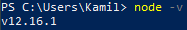
\includegraphics{images/node_version.png}
	\caption{Rezultat polecenia \textit{node -v}}\label{nodeversion}
\end {figure}

\section{Struktura oprogramowania}

System składa się z kilku modułów, dlatego dostarczone oprogramowanie jest podzielone na kilka folderów. Struktura folderów została przedstawiona na rysunku \ref{foldery}.

\begin{figure}[h]
	\centering
	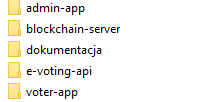
\includegraphics[width=\textwidth]{images/foldery.png}
	\caption{Struktura folderów}\label{foldery}
\end {figure}

Foldery przechowują następujące moduły:
\begin{itemize}
  \item dokumentacja przechowuje dokumentację projektu,
	\item admin-app przechowuje aplikację przeglądarkową administratora,
	\item voter-app przechowuje aplikację przeglądarkową użytkownika,
	\item e-voting-api przechowuje aplikację serwerową dostarczającą API systemu,
	\item blockchain-server przechowuje program, który realizuje działanie węzła w sieci Blockchain.
\end{itemize}

\section{Uruchamianie modułów}
 
Za pomocą menadżera pakietów NPM uruchamiane są poszczególne moduły systemu. Aby uruchomić dany moduł należy otworzyć katalog z tym modułem. W katalogu znajduje się plik \textit{package.json}, który zawiera konfigurację i skrypty uruchamiające program. Programy uruchamia się za pomocą poleceń dostarczanych przez pakiet NPM, które należy wpisać w konsoli. Konsola musi być uruchomiona w folderze z plikiem \textit{package.json}.
 
Moduły \textit{admin-app} i \textit{voter-app} uruchamiane są za pomocą polecenia \textit{npm-start}. Aplikacja \textit{admin-app} w środowisku lokalnym uruchamiana jest pod adresem \url{http://localhost:4000}, a aplikacja \textit{voter-app} pod adresem \url{http://localhost:3000}.
 
Podczas uruchamiania aplikacji serwerowych, należy określić port, na którym widoczny będzie określony serwer.
 
Aplikacja serwerowa \textit{e-voting-api} jest domyślnie uruchamiana na porcie 8080, jednak można to zmienić za pomocą następującego polecenia:
 
\begin{equation}
	\textit{\$env:PORT=NUMER\_PORTU; npm start}.
\end{equation}

Użycie tego polecenia jest obligatoryjne podczas uruchamiania węzła sieci Blockchain, ponieważ węzeł nie uruchamia się na domyślnym porcie. W celu uruchomienia węzła należy wybrać dowolny nieużywany port komputera.
 
Podczas uruchamiania węzła sieci Blockchain można wybrać algorytm konsensusu, który będzie wykorzystywał dany węzeł. Pełne polecenie uruchamiające węzeł Blockchain wygląda następująco:

\begin{equation}
	\textit{\$env:PORT=NUMER\_PORTU; \$env:CONSENSUS=KOD; npm start}.
\end{equation}

W polu \textit{KOD} należy wpisać kod algorytmu. Dostępne są dwa kody: \textit{POA} i \textit{POW}. Kod \textit{POA} odpowiada algorytmowi \textit{Proof of Authority}, a kod \textit{POW} algorytmowi \textit{Proof of Work}. W przypadku podania błędnego kodu lub jego braku, domyślnym algorytmem używanym przez węzeł jest \textit{Proof of Authority}.

\newpage

\section{Aplikacja administratora}

Aplikacja administratora jest najbardziej rozbudowanym elementem systemu. W tym podrozdziale przedstawiono dostępne scenariusze obsługi tej aplikacji.

\subsection{Logowanie}

Wszystkie funkcjonalności administratora dostępne są po zalogowaniu. Dlatego na stronie administratora pierwszym dostępnym widokiem jest formularz logowania (rys. \ref{adminlogin}).

\begin{figure}[h]
	\centering
	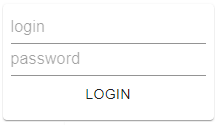
\includegraphics{images/adminlogin.png}
	\caption{Formularz logowania administratora.}\label{adminlogin}
\end {figure}

Po zalogowaniu ukazuje się strona administratora. Nawigacja po stronie administratora odbywa się za pomocą górnego paska nawigacji (rys. \ref{adminnav}). Z paska nawigacji można przejść do listy wyborców (\textit{Voters}), listy wyborów (\textit{Elections}) i panelu konfiguracji sieci Blockchain (\textit{Servers}). Na pasku nawigacji znajduje się również przycisk służący do wylogowania administratora z aplikacji (\textit{Logout}).

\begin{figure}[h]
	\centering
	
\includegraphics[width=\textwidth]{images/adminnav.png}
	\caption{Pasek nawigacji administratora.}\label{adminnav}
\end {figure}

\newpage

\subsection{Lista wyborców}

Lista wyborców dostarcza informacje o wyborcach utworzonych w systemie. Cały widok przedstawia rysunek \ref{voterslist}. Przycisk \textit{Create Voter} pozwala na dodanie nowego wyborcy do systemu. Po kliknięciu tego przycisku pojawia się okno \ref{addvoter}, które zawiera formularz dodawania nowego wyborcy. Do formularza należy wpisać dane nowego wyborcy.

\begin{figure}[h]
	\centering
	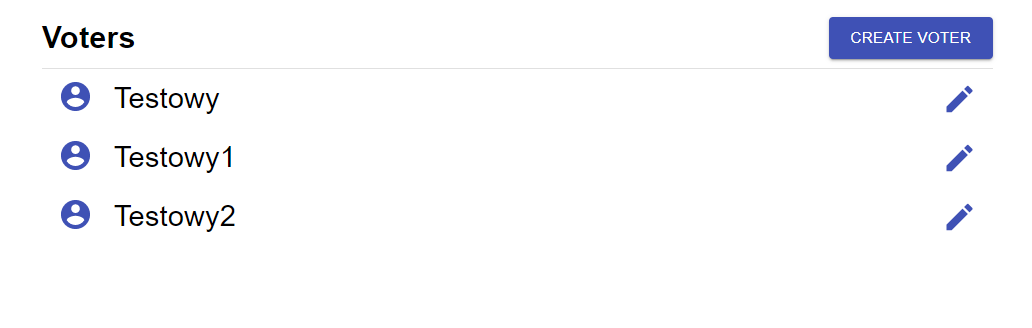
\includegraphics[width=\textwidth]{images/voterslist.png}
	\caption{Lista wyborców.}\label{voterslist}
\end {figure}

\begin{figure}[h]
	\centering
	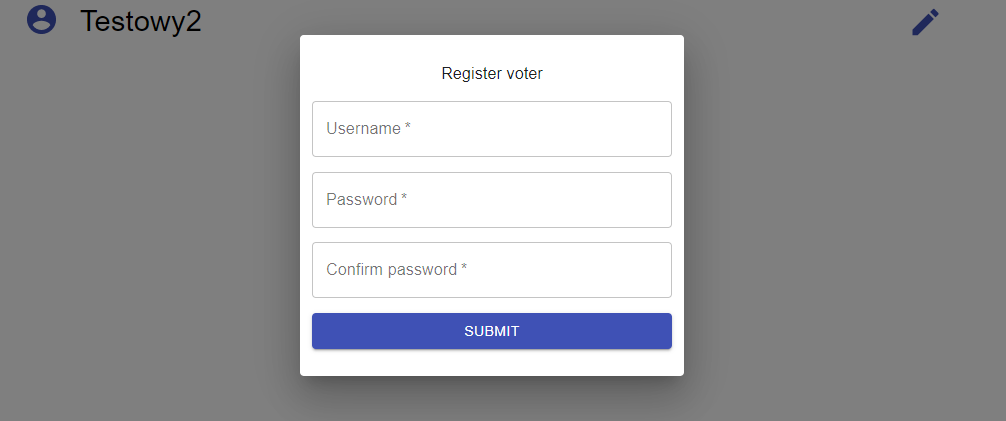
\includegraphics[width=\textwidth]{images/addvoter.png}
	\caption{Okno dodawania wyborcy.}\label{addvoter}
\end {figure}

\newpage

\subsection{Konfiguracja sieci Blockchain}

Administrator posiada interfejs pozwalający na tworzenie sieci Blockchain. Węzły Blockchain to oprogramowanie działające na pojedynczym serwerze. Za pomocą konfiguratora, administrator systemu może połączyć się z danym węzłem i połączyć z nim inne serwery. Interfejs jest dostępny po kliknięciu na pasku nawigacji opcji \textit{Servers}. Rysunek \ref{findnode} przedstawia wyszukiwarkę węzłów Blockchain. W pole \textit{Server url} należy wpisać adres serwera, na którym pracuje węzeł sieci Blockchain.

\begin{figure}[h]
	\centering
	
\includegraphics[width=\textwidth]{images/findnode.png}
	\caption{Wyszukiwarka węzłów.}\label{findnode}
\end {figure}

Pomyślne połączenie sygnalizowane jest zmianą koloru przycisku \textit{check}, tak jak na rysunku \ref{nodeconfig}. Na rysunku widać również zakładkę \textit{Peers}, która wyświetla wszystkie połączone węzły. Po podłączeniu do węzła administrator uzyskuje dostęp, do możliwości połączenia ze sobą dwóch węzłów. Do tego służy pole z etykietą \textit{Server url}, znajdujące się pod zakładką \textit{Peers}.

\begin{figure}[h]
	\centering
	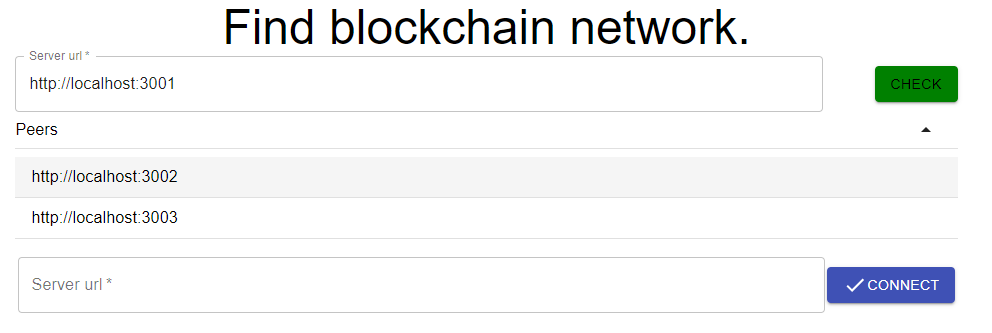
\includegraphics[width=\textwidth]{images/ndoeconfig.png}
	\caption{Konfiguracja podłączonego węzła.}\label{nodeconfig}
\end {figure}

W taki sposób można łączyć węzły i tworzyć sieci Blockchain. Bardzo ważne jest, aby każdy węzeł był połączony z węzłem głównym, który komunikuje się z API systemu.

\subsection{Lista wyborów}

Widok prezentujący listę wyborów pozwala na uzyskanie dostępu do menedżera wyborów, opcji tworzenia nowych wyborów i usunięcia wyborów. Rysunek \ref{electionlist} przedstawia omawiany widok. Ikona kosza pozwala na usunięcie wyborów, jeżeli wyniki wyborów są opublikowane. Ikona długopisu pozwala na zarządzanie wyborami. Przycisk \textit{Create election} przenosi użytkownika do konfiguratora wyborów, który pozwala na tworzenie nowych wyborów.

\begin{figure}[h]
	\centering
	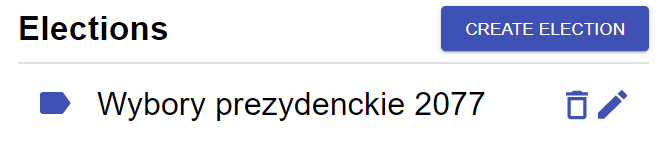
\includegraphics[width=\textwidth]{images/electionlist.png}
	\caption{Widok listy wyborów.}\label{electionlist}
\end {figure}

\subsection{Konfiguracja wyborów}

Konfiguracja wyborów to dosyć długi proces, dlatego został on podzielony na kilka etapów. Widok na rysunku \ref{votesconfig1} przedstawia pierwszy etap konfiguracji. W tym etapie administrator musi wypełnić formularz. W formularzu należy wpisać tytuł wyborów, opis, datę rozpoczęcia, datę zakończenia i adres głównego serwera sieci Blockchain, który jest punktem dostępu do całej sieci.

\begin{figure}[h]
	\centering
	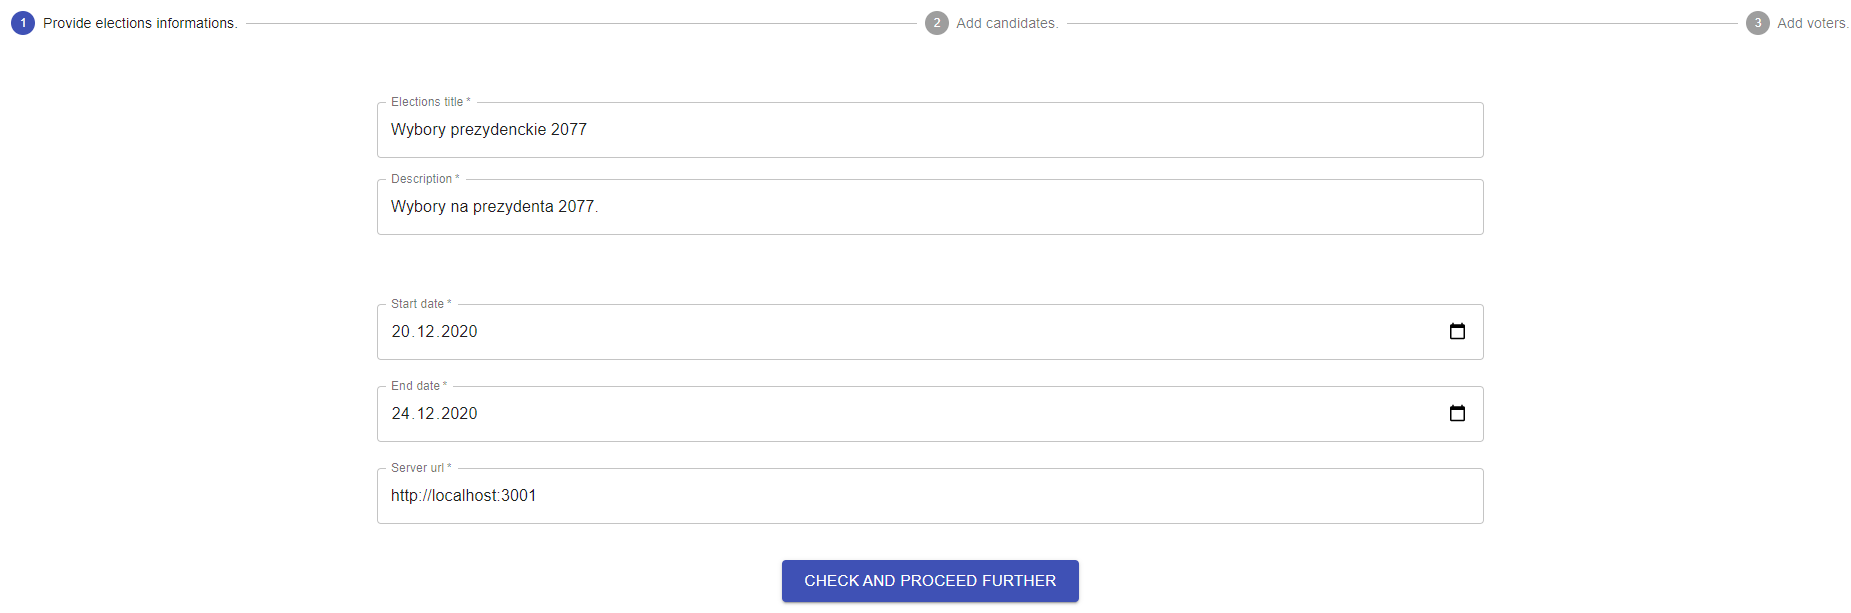
\includegraphics[width=\textwidth]{images/votesconfig1.png}
	\caption{Konfiguracja wyborów etap pierwszy.}\label{votesconfig1}
\end {figure}

Po wypełnieniu formularza należy kliknąć przycisk \textit{Check and proceed further}. Aplikacja sprawdzi poprawność formularza i poinformuje o błędach (rys. \ref{votesconfigerror}) lub wyświetli następny widok.

\begin{figure}[h]
	\centering
	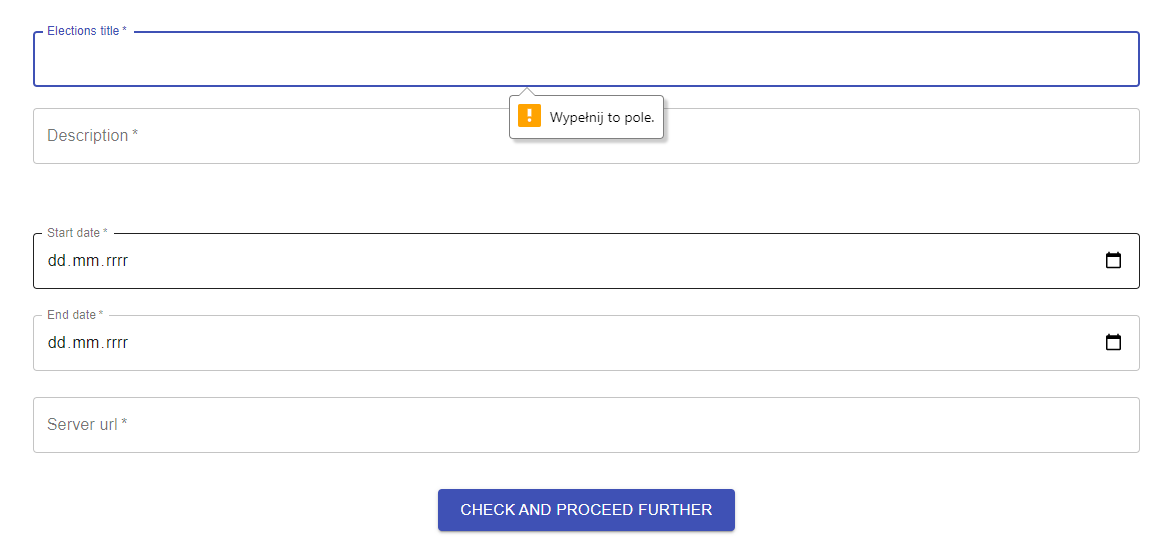
\includegraphics[width=\textwidth]{images/votesconfigerror.png}
	\caption{Wyświetlanie błędów formularza.}\label{votesconfigerror}
\end {figure}

Następnym widokiem jest formularz pozwalający na utworzenie kandydatów. Widok został przedstawiony na rysunku \textit{votescandidate}. Formularz jest zbudowany z dwóch pól tekstowych \textit{Candidate} i \textit{Description}, w których należy umieścić nazwę kandydata i jego opis. Dodatkowo w skład formularza wchodzą przyciski oznaczone plusem i minusem. Minus usuwa okno, a plus dodaje nowe okno do formularza. Przejście do następnego widoku następuje po kliknięciu przycisku \textit{Next}. Dodatkowo można powrócić do widoku pierwszego za pomocą przycisku \textit{Previous}.
\newpage

\begin{figure}[h]
	\centering
	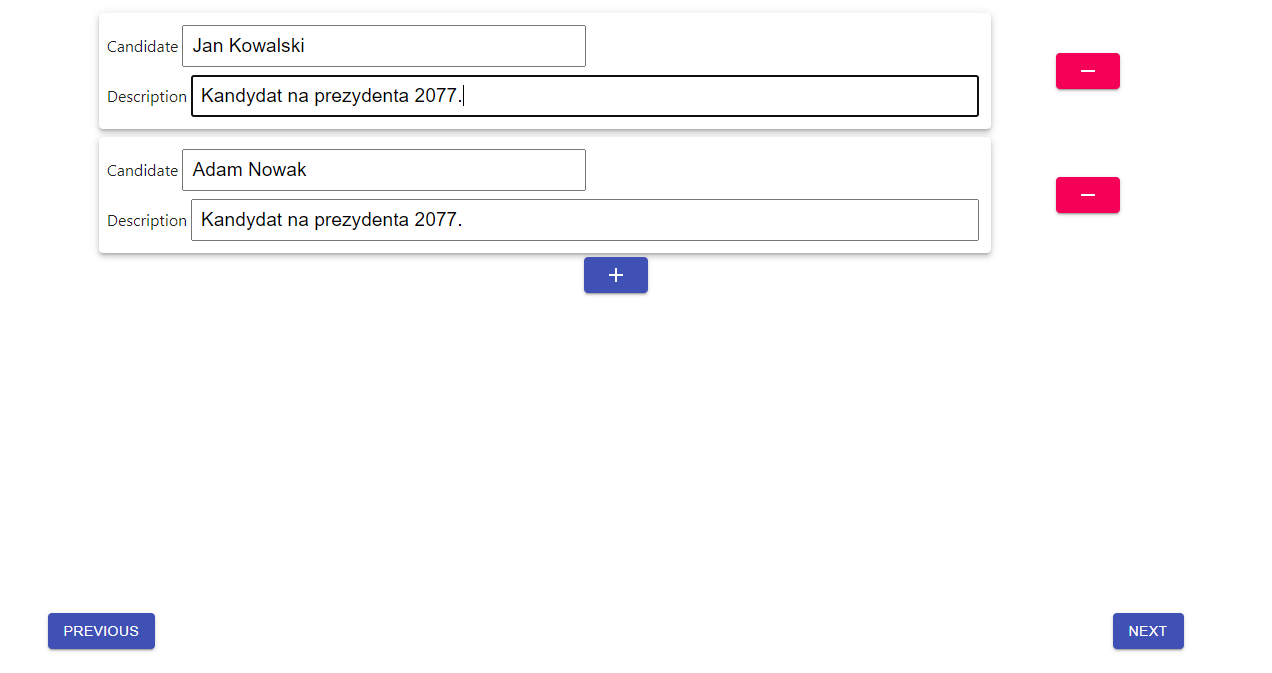
\includegraphics[width=\textwidth]{images/votescandidate.png}
	\caption{Formularz dodawania kandydatów. Etap drugi}\label{votescandidate}
\end {figure}

Następnym i ostatnim krokiem jest przypisanie wyborców do wyborów. Rysunek \ref{choosevoters} przedstawia formularz dodawania wyborców. Wyborców dodaje się poprzez zaznaczenie ich na liście. Żeby zakończyć proces konfiguracji wyborów należy kliknąć przycisk \textit{Submit}.

\begin{figure}[H]
	\centering
	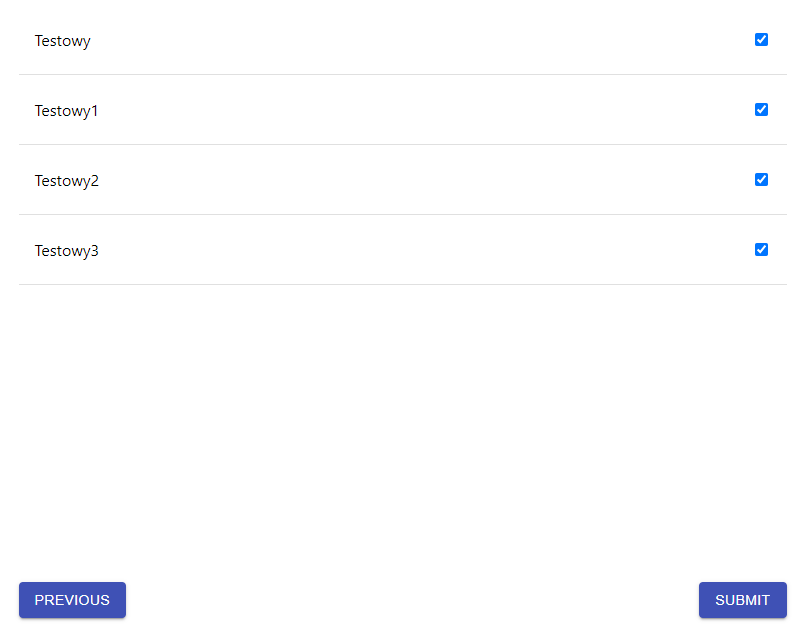
\includegraphics[width=\textwidth]{images/choosevoters.png}
	\caption{Lista dostępnych wyborów.}\label{choosevoters}
\end {figure}

Po utworzeniu wyborów następuje przeniesienie do widoku z listą wyborów (rys. \ref{electionsview}).

\begin{figure}[h]
	\centering
	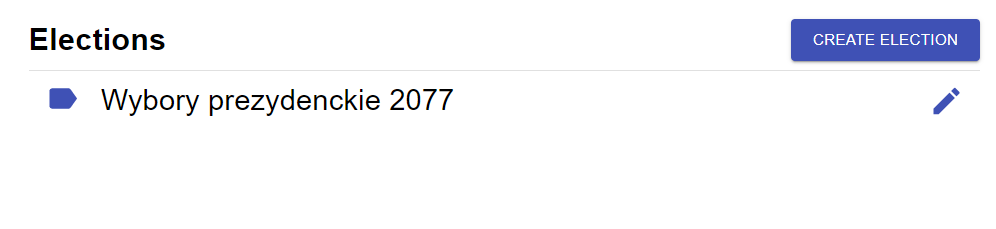
\includegraphics[width=\textwidth]{images/electionsview.png}
	\caption{Lista dostępnych wyborów.}\label{electionsview}
\end {figure}

\subsection{Nadzorowanie wyborów}

Żeby przejść do panelu nadzorowania wyborów, z poziomu widoku listy wyborów (rys. \textit{electionsview}) należy kliknąć ikonę edycji (rys. \ref{penicon}).

\begin{figure}[h]
	\centering
	
\includegraphics{images/penicon.png}
	\caption{Ikona edycji.}\label{penicon}
\end {figure}

Po kliknięciu przycisku ukazuje się menu zarządzania wyborami (rys. \ref{electionmanager}). Na górze menu widać rozszerzenie paska nawigacji, które pozwala na przełączanie się pomiędzy funkcjami menadżera wyborów. Widokiem, który ukazuje się jako pierwszy jest komponent o tytule \textit{Status}. Ten komponent wyświetla tytuł i opis wyborów, a także adres głównego węzła sieci Blockchain odpowiedzialnego za dane wybory. Na rysunku \ref{electionmanager} widać przycisk \textit{Change Url}, którego kliknięcie aktywuje pole tekstowe z etykietą \textit{Server Url} (rys. \ref{changeurl}). W pole tekstowe należy wpisać adres nowego serwera sieci Blockchain, który ma być traktowany jako węzeł główny. Zmiana serwera następuje po kliknięciu przycisku \textit{Submit}. Pozwala to na zmianę serwera, jeżeli używany serwer uległ awarii.

\begin{figure}[h]
	\centering
	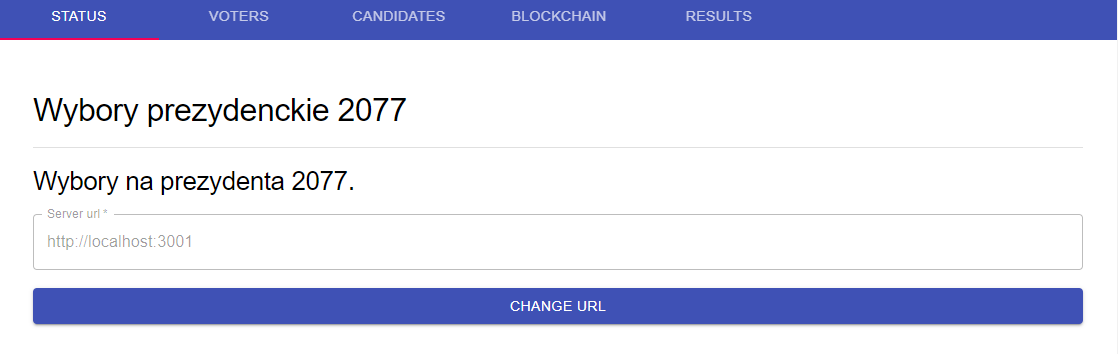
\includegraphics[width=\textwidth]{images/electionmanager.png}
	\caption{Komponent Status.}\label{electionmanager}
\end {figure}

\begin{figure}[H]
	\centering
	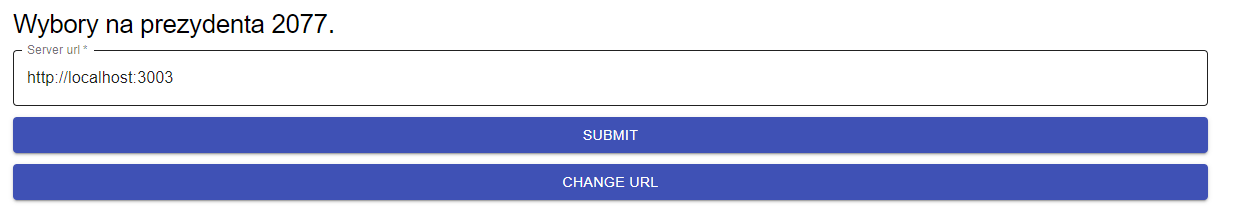
\includegraphics[width=\textwidth]{images/changeurl.png}
	\caption{Zmiana adresu serwera.}\label{changeurl}
\end {figure}

Kolejne komponenty, które można wyświetlić poprzez pasek nawigacji (rys. \ref{electionmanager}) to \textit{Voters} i \textit{Candidates}. \textit{Voters} prezentuje listę wyborców przypisanych do głosowania, a \textit{Candidates} listę kandydatów. Są to komponenty informacyjne, które przedstawiono na rysunkach \ref{infovoters} i \ref{infocandidates}.

\begin{figure}[H]
	\centering
	
\includegraphics{images/infocandidates.png}
	\caption{Lista kandydatów.}\label{infocandidates}
\end {figure}

\begin{figure}[H]
	\centering
	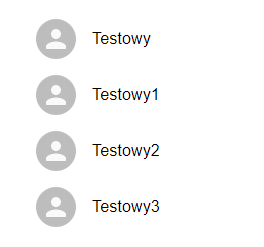
\includegraphics{images/infovoters.png}
	\caption{Lista wyborców.}\label{infovoters}
\end {figure}

Komponent Blockchain (rys. \ref{bcstatus}) zawiera informacje dotyczące liczby stworzonych bloków (\textit{Blocks created}) i węzłów (\textit{Nodes}) w sieci Blockchain. 

\begin{figure}[H]
	\centering
	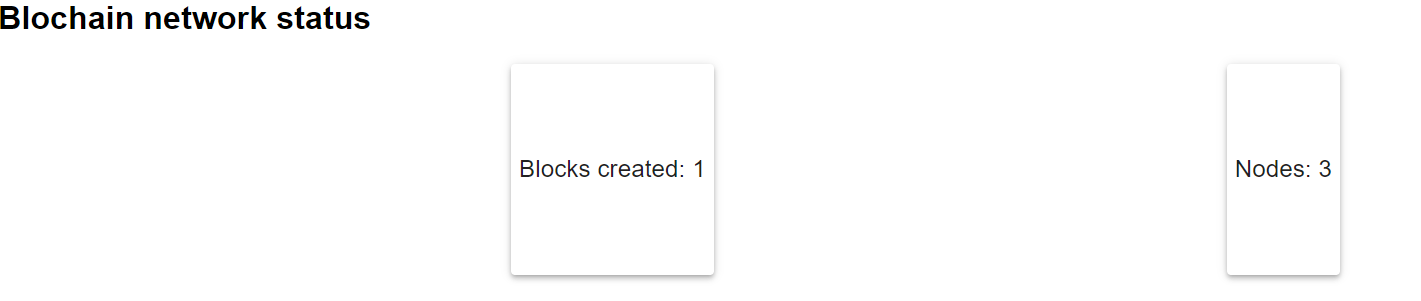
\includegraphics[width=\textwidth]{images/bcstatus.png}
	\caption{Dane dotyczące sieci Blockchain.}\label{bcstatus}
\end {figure}

Ostatnim komponentem menadżera wyborów jest
Results
. Ten komponent od-
powiada za publikację wyników wyborów. Wyniki wyborów są tajne, dla każdego
aktora systemu, do momentu ich opublikowania. Po otwarciu komponentu, jeżeli
wyniki wyborów nie zostały opublikowane wyświetlony zostaje przycisk \ref{publish}. Po
kliknięciu tego przycisku wyniki wyborów zostaną opublikowane i pobierane z
serwera. Wyświetlany jest wykres słupkowy prezentujący wyniki wyborów (rys.
\ref{adminelectionresult}).

\begin{figure}[H]
	\centering
	
\includegraphics{images/publish.png}
	\caption{Przycisk publikowania wyborów.}\label{publish}
\end {figure}

\begin{figure}[H]
	\centering
	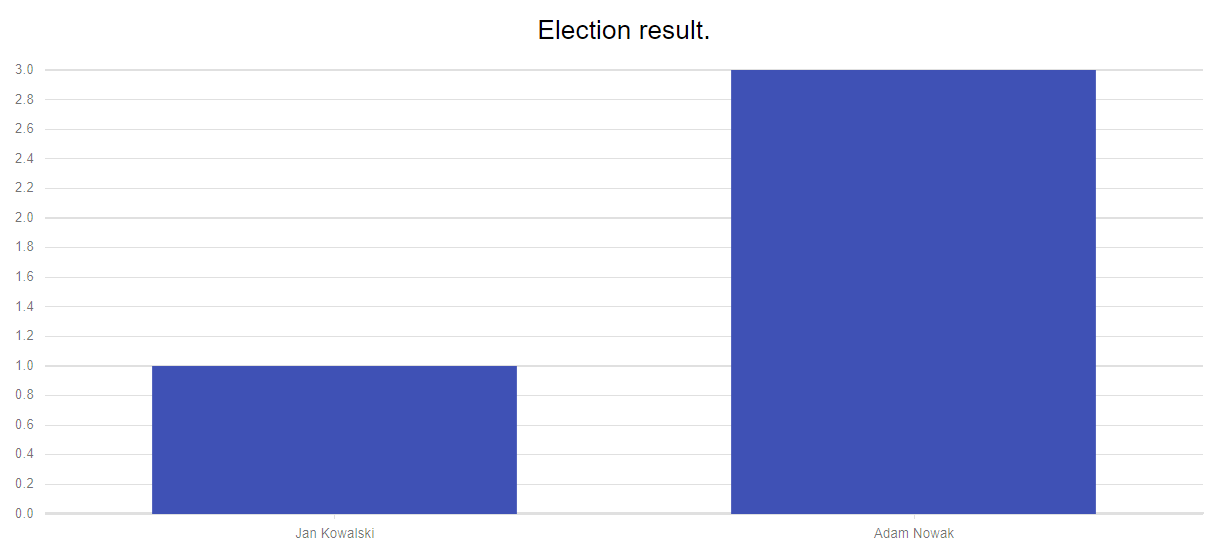
\includegraphics[width=\textwidth]{images/adminelectionresult.png}
	\caption{Diagram słupkowy prezentujący wyniki.}\label{adminelectionresult}
\end {figure}
\newpage
%%%%%%%%%%%%%%%%%%%%%%%%%%%%%%%%%%%%%%%%%%%%%%%%%%%%%%%%%%
\section{Aplikacja użytkownika}

Aplikacja użytkownika dostarcza interfejs pozwalający na wysłanie głosu i odczytanie wyników wyborów. Ten podrozdział przedstawia scenariusze obsługi aplikacji wyborcy.
 
\subsection{Logowanie}

Dostęp do zasobów wyborcy wymaga zalogowania. W celu zalogowania się należ kliknąć przycisk \textit{login}, który znajduję w prawym górnym rogu, na pasku nawigacji (rysunek \ref{navlogin}).

\begin{figure}[h]
	\centering
	
\includegraphics[width=\textwidth]{images/navlogin.png}
	\caption{Pasek nawigacji.}\label{navlogin}
\end {figure}

Po kliknięciu przycisku \textit{login} na ekranie pojawia się okno, które wymaga podania loginu i hasła wyborcy. Okno przedstawiono na rysunku \ref{userlogin}. Jeżeli dane logowania są poprawne, to następuje przeniesienie do strony wyborcy (rys. \ref{manual}).
 
\begin{figure}[h]
	\centering
	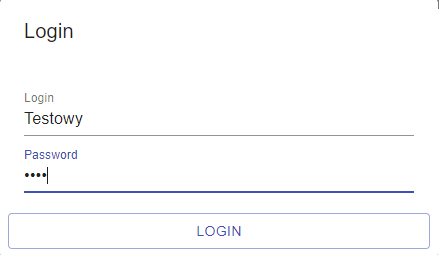
\includegraphics{images/userlogin.png}
	\caption{Okno logowania.}\label{userlogin}
\end {figure}

\begin{figure}[h]
	\centering
	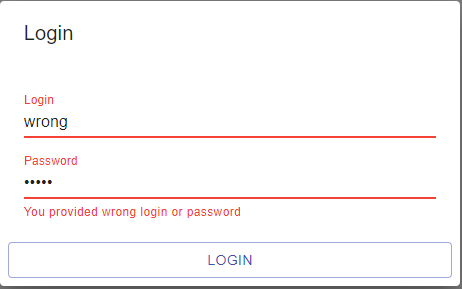
\includegraphics{images/errorlogin.png}
	\caption{Obsługa błędnych danych logowania.}\label{wronglogin}
\end {figure}

Jeżeli użytkownik poda błędne dane logowania, to zostanie o tym poinformowany poprzez wyświetlenie stosownego komunikatu w oknie logowania (rys. \ref{wronglogin}). 

\newpage

Wylogowanie wymaga kliknięcia przycisku \textit{Logout} w prawym górnym rogu strony wyborcy (rys. \ref{manual}).

\subsection{Instrukcja obsługi}

Instrukcja obsługi, to krótki opis wykonywania podstawowych akcji na stronie użytkownika. Można do niej przejść klikając \textit{help} na pasku nawigacji (rys. \ref{manual}). Informacje zawarte w instrukcji dotyczą: wyboru głosowania, procesu głosowania i wyników wyborów.

\begin{figure}[H]
	\centering
	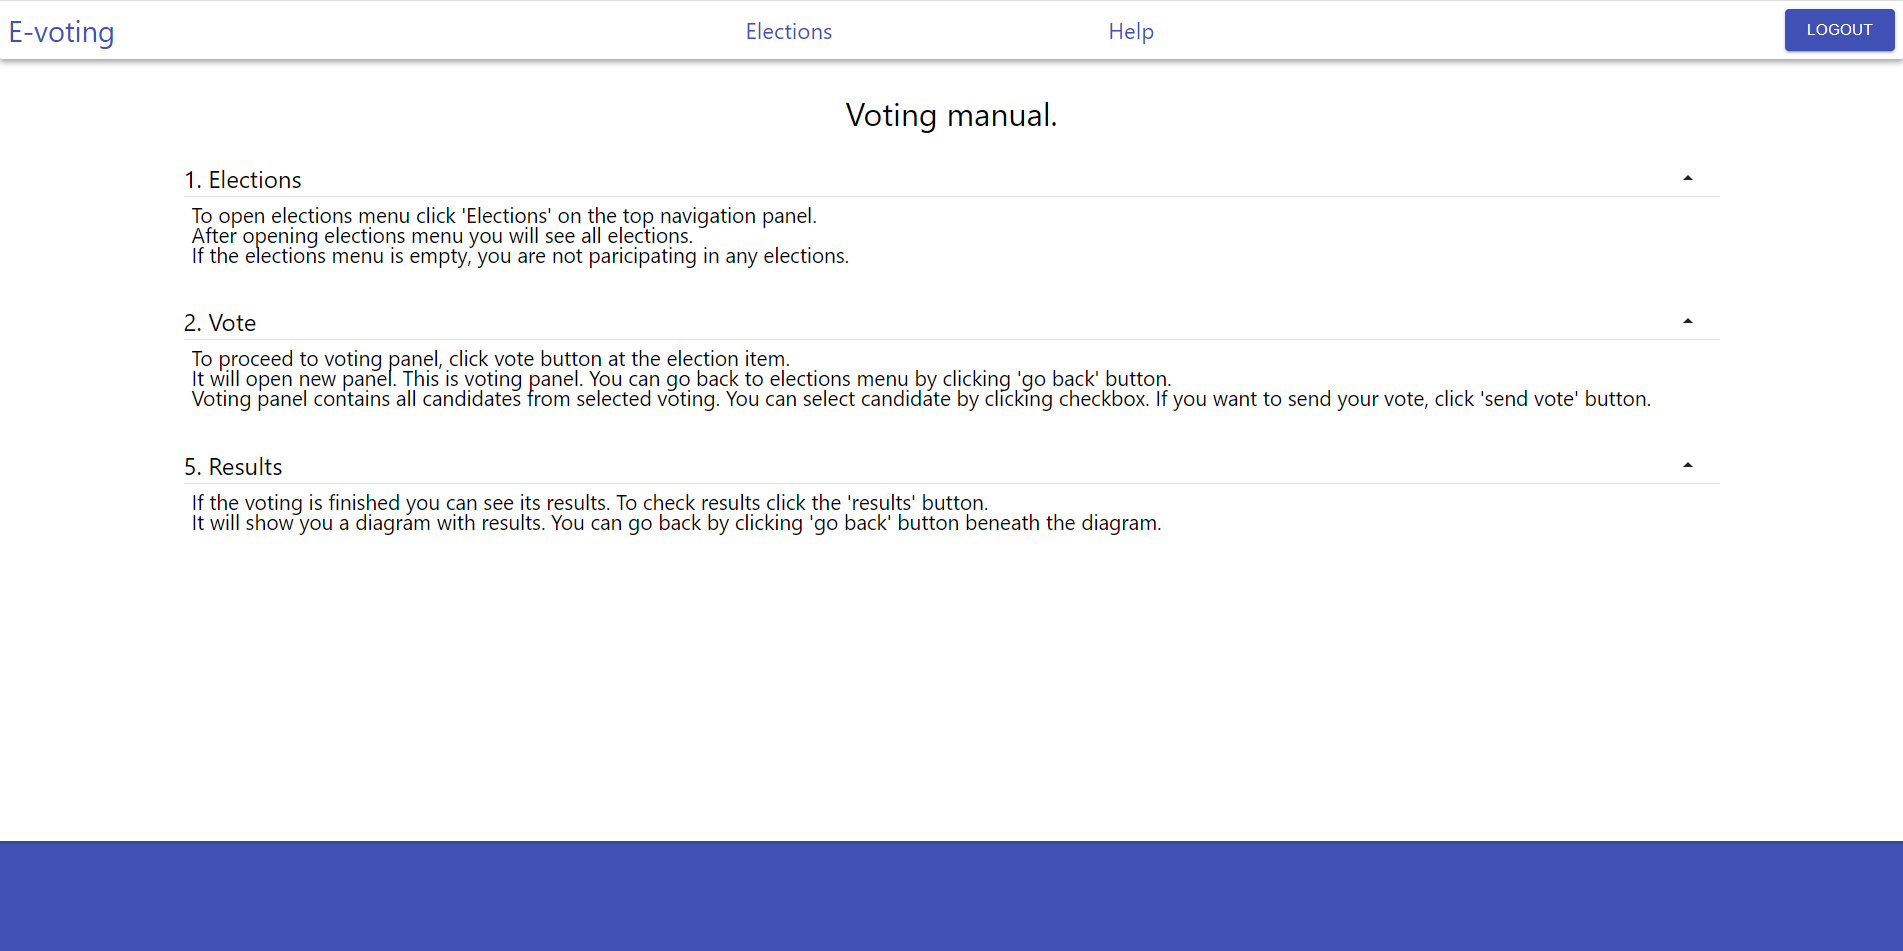
\includegraphics[width=\textwidth]{images/manual.png}
	\caption{Strona wyborcy. Instrukcja obsługi.}\label{manual}
\end {figure}

\newpage

\subsection{Głosowanie}

Głosowanie dostępne jest po kliknięciu \textit{Elections} na pasku nawigacji. Po wybraniu tej opcji z paska nawigacji następuje przekierowanie do strony, której zawartość przedstawiona jest na rysunku \ref{electionwindow}. Jeżeli wyborca bierze udział w większej liczbie wyborów, to będzie miał do wyboru więcej opcji, niż na rysunku \ref{electionwindow}.

Okno  przedstawione na rysunku \ref{electionwindow} zawiera przycisk oznaczony \textit{Vote}. Kliknięcie tego przycisku przenosi użytkownika do głównego panelu wyborów \ref{votescreen}. W tym miejscu wyborca dokonuje wyboru kandydata i przesyła swój głos, po klinięciu przycisku \textit{Send Vote}. Wyborca może cofnąć widok, do poprzedniego widoku, za pomocą przycisku \textit{Go Back}.

\begin{figure}[H]
	\centering
	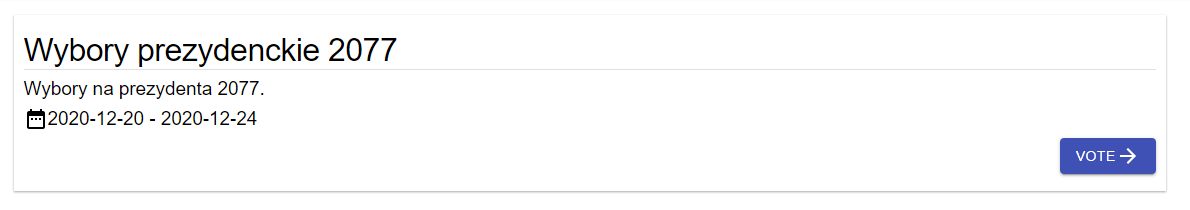
\includegraphics[width=\textwidth]{images/electionwindow.png}
	\caption{Okno wyborcze.}\label{electionwindow}
\end {figure}

\begin{figure}[H]
	\centering
	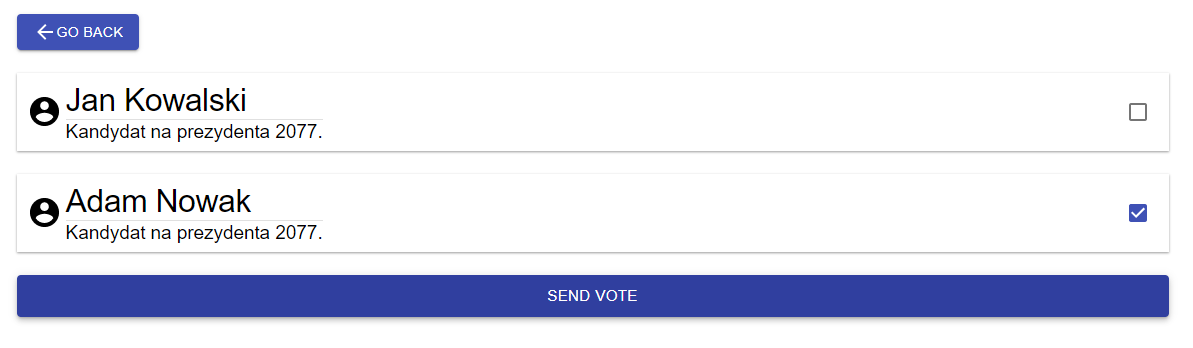
\includegraphics[width=\textwidth]{images/votescreen.png}
	\caption{Panel wyborów.}\label{votescreen}
\end {figure}

Po wysłaniu głosu na ekranie pojawia się powiadomienie \ref{votesuccess} i następuje przeniesienie do widoku \ref{votesent}.

\begin{figure}[H]
	\centering
	
\includegraphics{images/votesuccess.png}
	\caption{Pomyślnie wysłany głos.}\label{votesuccess}
\end {figure}

\begin{figure}[H]
	\centering
	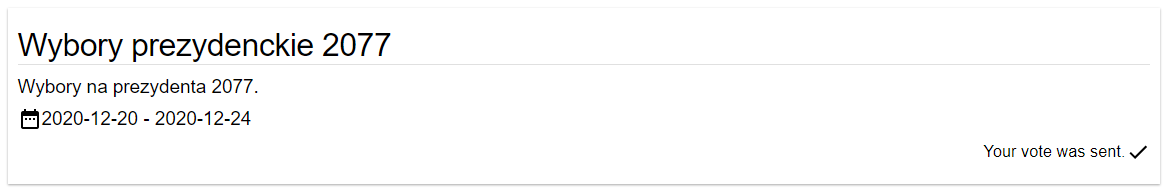
\includegraphics[width=\textwidth]{images/votesent.png}
	\caption{Okno wyborów. Po zagłosowaniu.}\label{votesent}
\end {figure}

\subsection{Wyniki}

Dostęp do wyników wyborów uzyskiwany jest po ogłoszeniu wyników. Wybory, których wyniki są dostępne oznaczone są tak jak na rysunku \ref{voterresults}. Okno zawiera przycisk \textit{results}, którego kliknięcie przenosi użytkownika do okna \ref{resultdiagram}. Wykres jest podobny do wykresu administratora (rys. \ref{adminelectionresult}). Wrócić do poprzedniego widoku można za pomocą przycisku pod wykresem \textit{Go Back}.

\begin{figure}[H]
	\centering
	
\includegraphics[width=\textwidth]{images/voterresults.png}
	\caption{Okno wyborów. Po ogłoszeniu wyników.}\label{voterresults}
\end {figure}

\begin{figure}[H]
	\centering
	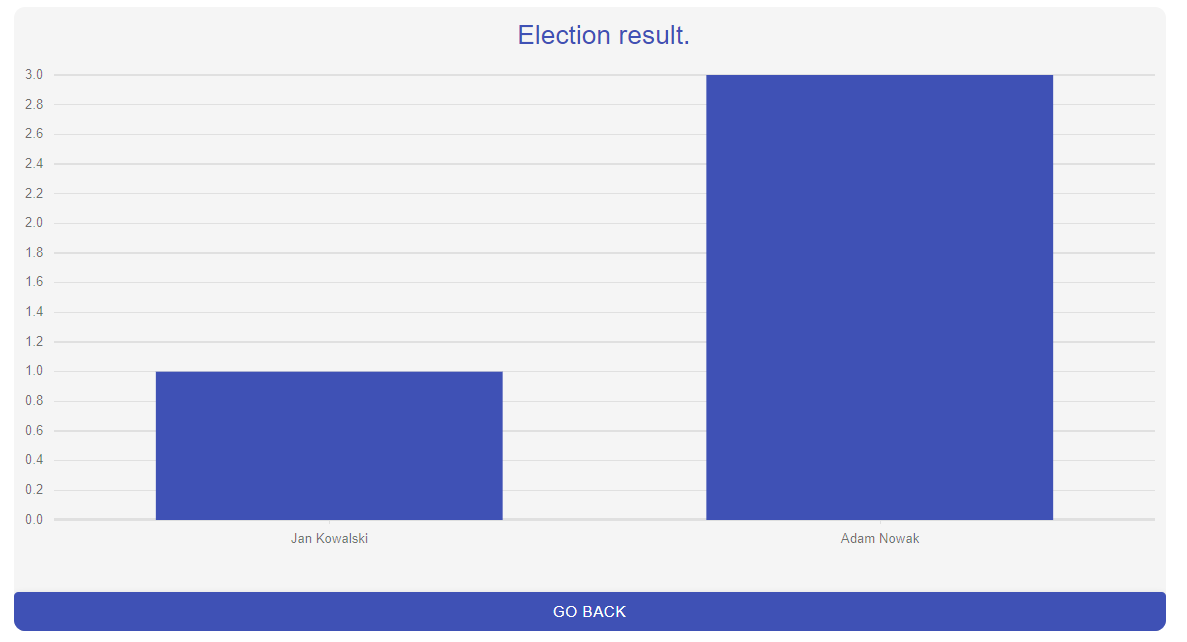
\includegraphics[width=\textwidth]{images/resultdiagram.png}
	\caption{Wykres wyników wyborów.}\label{resultdiagram}
\end {figure}

%%%%%%%%%%%%%%%%%%% Specyfikacja wewnętrzna %%%%%%%%%%%%%%%%%%%%%%%%%%%%

\chapter{Specyfikacja wewnętrzna}

W tym rozdziale umieszczono wszystkie informacje dotyczące architektury systemu, wykorzystanych struktur danych, algorytmów i wykorzystania wzorców projektowych.
 
\section{Architektura systemu}
Podrozdział architektura systemu zawiera przegląd komponentów systemu, także nakreśla idee projektu. Podrozdział podzielono na dwie części. Pierwsza część dotyczy całego systemu, natomiast druga opisuje charakterystykę sieci Blockchain.
 
\subsection{Architektura pełnego systemu}
 
System składa się z pięciu głównych komponentów:

\begin {itemize}
	\item aplikacja wyborcy - pozwala na dostęp do zasobów wyborcy,
	\item aplikacja administratora - umożliwia konfigurację wyborów, audytowanie wyborów, zarządzanie sieciami Blockchain i zarządzanie bazą danych,
	\item serwer z API - serwer, na którym uruchomione jest API. API dostarcza odpowiednie zasoby określonym użytkownikom i posiada dostęp do bazy danych,
	\item baza danych - przechowuje informacje dotyczące konfiguracji wyborów. Listy użytkowników, wyborów, kandydatów i określa relacje pomiędzy nimi. W bazie danych znajdują się również hasła użytkowników,
	\item sieć Blockchain - odpowiada za przechowywanie głosów i udostępnianie ich na życzenie administratora. Blockchain pełni również funkcje zabezpieczenia głosów.
\end {itemize}

Komponenty są przedstawione na rysunku \ref{komponenty}.

\begin{figure}[H]
    	\centering
	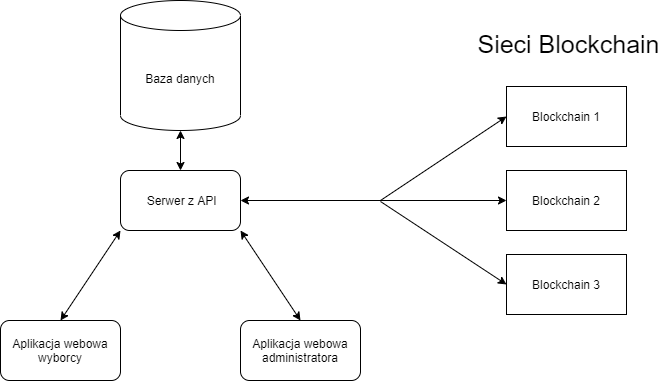
\includegraphics[width=\textwidth]{images/modules.png}
	\caption{Schemat przedstawiający komponenty systemu.}\label{komponenty}
\end {figure}

Taki podział systemu umożliwia wykorzystanie sieci Blockchain. Proces przeprowadzania wyborów jest scentralizowany, a sieć Blockchain, która odpowiada za zapisanie wyników wyborów jest rozproszona.
 
\subsection{Architektura sieci Blockchain}
 
Sieć Blockchain to grupa serwerów, które wymieniają się informacjami. Komunikacja głównie odbywa się w celu przesłania zawartości nowego bloku, synchronizacji danych i dodania nowego węzła do sieci.

Rysunek \ref{blockchainarch} przedstawia sieć Blockchain złożoną z pięciu węzłów. Wszystkie węzły połączone są ze sobą. W sieci można wyróżnić węzeł główny, którego zadaniem jest utrzymanie połączenia z REST API systemu wyborczego.

Drogą komunikacyjną pomiędzy REST API, a węzłem głównym przesyłane są głosy i żądania dotyczące wyniku wyborów oraz statusu sieci.

\begin{figure}[h]
  \centering
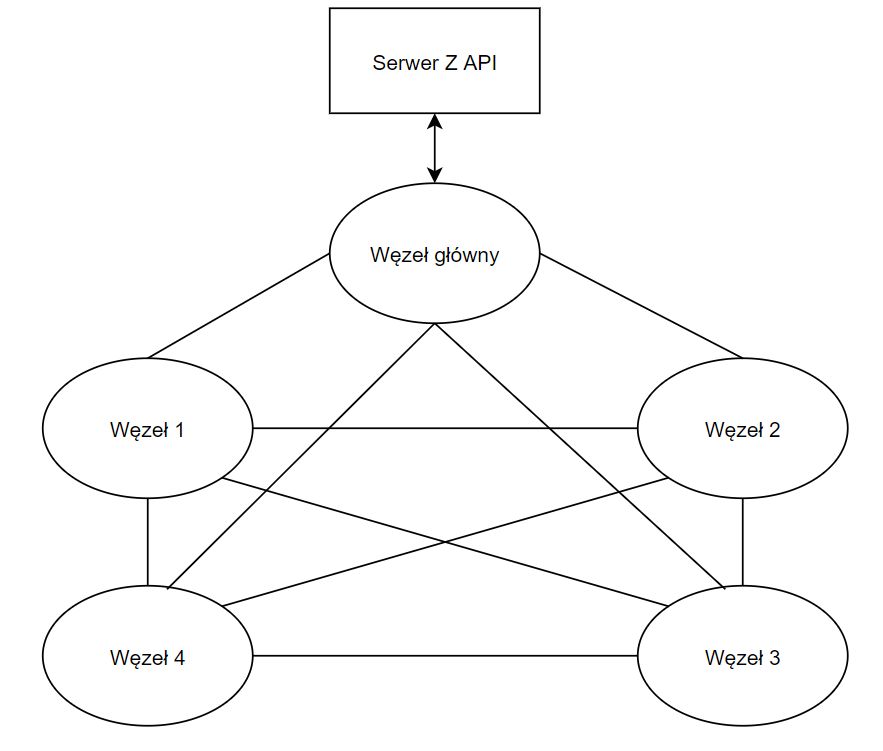
\includegraphics[width=\textwidth]{images/blockchainarch.png}
\caption{Schemat przedstawiający przykładową sieć Blockchain.}\label{blockchainarch}
\end {figure}

\newpage

\section{Struktury danych}
 
W systemie można wyróżnić dwie struktury danych, które w znaczny sposób wpływają na zachowanie systemu. W tym podrozdziale omówiono implementację i zastosowania tych struktur danych.
 
\subsection{Łańcuch bloków}
 
Za dostarczenie odpowiedniej struktury łańcucha bloków odpowiedzialne są klasy \textit{Block} i \textit{ChainRepository}. Listing \ref{Block.ts} przedstawia klasę \textit{Block}, która jest reprezentacją pojedynczego bloku. Każdy blok jest odpowiedzialny za przechowywanie głosu wyborczego. Głos jest przechowywany w polu \textit{data}. Pole \textit{timestamp} przechowuje datę utworzenia bloku w łańcuchu. W łańcuchu bloków, każdy blok posiada odniesienie do \textit{hash'u} poprzedniego bloku. W przedstawionej implementacji zajmuje się tym pole \textit{prevHash}. Klasa \textit{Block} posiada również pole \textit{nonce}, którego zastosowanie dotyczy algorytmu \textit{Proof of Work}.

\newpage

\begin{lstlisting}[style=ES6, caption={Klasa \textit{Block}.},label={Block.ts}]
class Block {
  index: number
  timestamp: string
  nonce: number
  prevHash: string
  data: string

  constructor (index: number,
 		timestamp: string,
 		nonce: number,
 		prevHash: string,
	 	data: string) {
    this.index = index
    this.timestamp = timestamp
    this.nonce = nonce
    this.prevHash = prevHash
    this.data = data
  }
}
\end{lstlisting}

Klasa \textit{ChainRepository} (przedstawiona w listingu \ref{ChainRepository.ts}) odpowiada za przechowywanie łańcucha bloków i jego udostępnianie. Aby zapewnić spójność danych, ułatwienie dostępu i ograniczenie zużycia pamięci, w programie istnieje tylko jedna instancja tej klasy. W tym celu wykorzystano wzorzec projektowy Singleton. Z punktu widzenia łańcucha bloków istotne jest pole \textit{chain}. Jest to tablica bloków. Klasa udostępnia metodę \textit{addBlock}, która pozwala na dodawanie nowego bloku na początek tablicy, zgodnie z regułą tworzenia łańcucha bloków. Dodatkowo klasa posiada prywatną metodę \textit{createGenesisBlock}, która tworzy pierwszy blok łańcucha, którego zawartość nie przechowuje istotnych danych. Metoda wywoływana jest podczas tworzenia instancji \textit{ChainRepository}.

\newpage

\begin{lstlisting}[style=ES6, caption={Klasa \textit{ChainRepository}.}, label={ChainRepository.ts}]
class ChainRepository {
  public static instance: ChainRepository
  private chain: Block[]

  private constructor () {
    this.chain = new Array<Block>()
    this.createGenesisBlock()
  }

  public static getInstance (): ChainRepository {
    if (!ChainRepository.instance) {
      ChainRepository.instance = new ChainRepository()
    }
    return ChainRepository.instance
  }

  public addBlock (block: Block) {
    this.chain.push(block)
  }

  private createGenesisBlock () {
    const block 
	= new Block(this.chain.length, '0', 0, '0', 'genesis')

    this.chain.push(block)
  }
/* ... Getters and setters*/
}
\end{lstlisting}

Za zapewnienie poprawnego utworzenia nowego bloku odpowiedzialna jest metoda \textit{createNewBlock} (listing \ref{Blockchain1.ts}), która należy do klasy \textit{Blockchain}. Metoda przyjmuje następujące parametry: \textit{nonce}, \textit{prevBlock} i \textit{data}. Z parametru \textit{prevBlock} wyliczany jest \textit{hash}, za pomocą metody \textit{getHash}. Jest to \textit{hash} poprzedniego bloku, który przypisywany jest do pola \textit{prevHash} tworzonego bloku.

\newpage

\begin{lstlisting}[style=ES6, caption={Fragment klasy Blockchain.},label={Blockchain1.ts}]
abstract class Blockchain {
  protected blockchain: ChainRepository

  public createNewBlock (nonce: number,  prevBlock: Block, 
					data: string): Block {
    const blockchain = this.blockchain.getChain()
    const chainLength = blockchain.length
    const prevHash = this.getHash(prevBlock)
    const date = Date.now().toString()

    const block = new Block(chainLength, date, nonce,
		 prevHash, data)

    return block
  }

  protected getHash (block: Block): string {
    const inputWord = block.toString()
    const hash = SHA256(inputWord).toString()
    return hash
  }
 /* ...  */
}
\end{lstlisting}

Tak skonstruowany blok jest gotowy do dodania do łańcucha. Dodawanie bloku jest realizowane za pomocą metody \textit{addBlock}, klasy \textit{ChainRepository}.

\subsection{Baza danych}

W projekcie wykorzystano relacyjną bazę danych. Taka struktura danych pozwala na uporządkowanie danych, w relacje pomiędzy tabelami. Rysunek \ref{database} przedstawia schemat relacyjnego modelu wykorzystanej bazy danych.

\begin{figure}[h]
    	\centering
	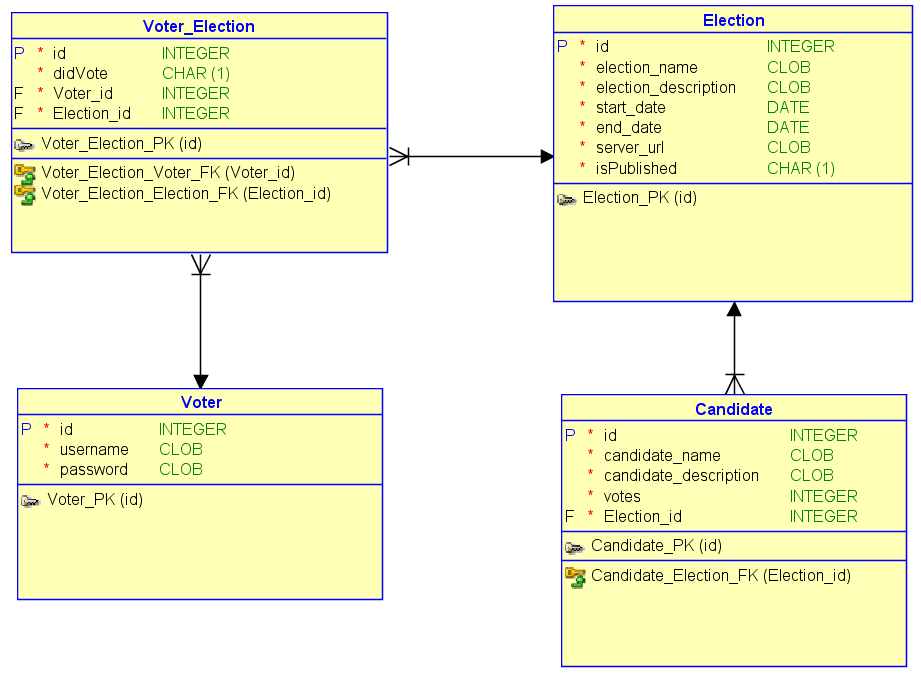
\includegraphics[width=\textwidth]{images/Relational.png}
	\caption{Schemat przedstawiający relacyjny schemat bazy danych.}\label{database}
\end {figure}

Bazę danych można podzielić na część odpowiadającą za przechowywanie konfiguracji wyborów oraz część przechowującą hasła i róle użytkowników. Tabele \textit{ADMIN} i \textit{VOTER} przechowują dane logowania aktorów systemu. Na podstawie tych tabel można dokonać autoryzacji użytkownika systemu i przydzielić mu odpowiednią rolę, która zapewnia dostęp do zasobów. Dodatkowo tabela \textit{VOTER} jest połączona relacją wiele do wielu z tabelą \textit{ELECTION}. W wyniku relacji wiele do wielu powstała tabela łącznikowa \textit{VOTER\_ELECTION}, która pozwala podzielić relację wiele do wielu, na dwie relacje jeden do wielu. Tabela \textit{VOTER\_ELECTION} pozwala na przypisanie wyborcy do odpowiednich wyborów. Dodatkowo tabela przechowuje informację o oddaniu głosu przez wyborcę, w polu \textit{DID\_VOTE}.
 
Pozostała część tabel odpowiada za przechowywanie danych dotyczących bezpośrednio wyborów. Zadaniem tabeli \textit{ELECTION} jest składowanie danych dotyczących konfiguracji wyborów. 

Konfiguracji mogą podlegać:
\begin{itemize}
	\item \textit{ELECTION\_NAME} - tytuł wyborów,
	\item \textit{ELECTION\_DESCRIPTION} - opis dotyczący wyborów,
	\item \textit{START\_DATE} - data rozpoczęcia wyborów,
	\item \textit{END\_DATE} - data zakończenia wyborów,
	\item \textit{SERVER\_URL} - adres zewnętrznego serwera sieci Blockchain, na który wysłane są głosy wyborców,
	\item kandydaci - zbiór kandydatów, którzy biorą udział w wyborach, jest reprezentowany jako relacja jeden do wielu z tabelą \textit{CANDIDATE}.
\end{itemize}

Dodatkowo w tabeli znajduje się również pole \textit{IS\_PUBLISHED} typu \textit{Boolean}, które odpowiada za oznaczenie stanu wyborów jako opublikowane lub nieopublikowane. System wykorzystuje tę informację do zakończenia wyborów i udostępnienia ich wyników.

Tabela \textit{CANDIDATE} reprezentuje kandydata, którego dane i opis definiują pola \textit{CANDIDATE\_NAME} i \textit{CANDIDATE\_DESCRIPTION}. Tabela posiada również pole \textit{VOTES}, które po zakończeniu wyborów uzupełniane jest o liczbę zdobytych głosów, przez danego kandydata.

\section{Algorytmy}

W podrozdziale Algorytmy opisano implementację algorytmów konsensusu, w sieci Blockchain. Węzeł sieci Blockchain może pracować w dwóch algorytmach konsensu: \textit{Proof of Work} lub uproszczonej wersji algorytmu \textit{Proof of Authority}. Każdy węzeł sieci Blockchain pozwala na wybranie algorytmu konsensusu, w którym będzie pracował. Algorytmy różnią się sposobem dodawania nowego bloku i synchronizacją sieci. Wybór algorytmu jest możliwy, poprzez wykorzystanie wzorca projektowego strategia. Implementacja tego wzorca projektowaego została opisana w rozdziale 6.4.

\subsection{Proof of Work}

Dodawanie nowego bloku w algorytmie \textit{Proof of Work} poprzedzone jest rozwiązaniem zagadki matematycznej. W listingu \ref{validateNonce} przedstawiono metodę \textit{validateNonce}, która zajmuje się weryfikacją rozwiązania zagadki.

\begin{lstlisting}[style=ES6, caption={Metoda \textit{validateNonce}.}, label={validateNonce}]
private validateNonce (
    lastNonce: number,
    nonce: number,
    prevHash: string
  ): boolean {
    const attempt = `${lastNonce}${nonce}${prevHash}`
    const hash = SHA256(attempt).toString()

    const isValid = hash.startsWith('000')
    return isValid
  }
\end{lstlisting}

Rozwiązanie zagadki matematycznej, to znalezienie odpowiedniej liczby (\textit{nonce}), która po dołączeniu do określonego stałego ciągu znaków i \textit{hash’owaniu} go, daje ciąg określonej liczby zer na początku. W przypadku tej implementacji są to trzy zera.
 
Metoda \textit{solveNonce} (listing \ref{solveNonce}) zajmuje się znalezieniem liczby \textit{nonce}. W pętli wywołana jest metoda \textit{validateNonce}, do momentu rozwiązania zagadki. Wraz z każdą iteracją pętli wykonywana jest inkrementacja zmiennej \textit{nonce}.
 
\begin{lstlisting}[style=ES6, caption={Metoda \textit{solveNonce}.}, label={solveNonce}]
private solveNonce (lastNonce: number, prevHash: string) {
    let nonce = 0

    while (!this.validateNonce(lastNonce, nonce, prevHash)) {
      nonce++
    }
    return nonce
  }
\end{lstlisting}

Dodawanie nowego bloku jest przeprowadzane w metodzie \textit{mine}. Metodę przedstawiono w listingu \ref{mine}.

\begin{lstlisting}[style=ES6, caption={Dodawanie nowego bloku. Metoda \textit{mine}.},label={mine}]
  public mine (data: any) {
    const blockchain = this.blockchain.getChain()
    const lastBlock = blockchain[blockchain.length - 1]
    const prevHash = this.getHash(lastBlock)
    const nonce = this.solveNonce(lastBlock.nonce, prevHash)

    const newBlock = this.createNewBlock(nonce, lastBlock, data)
    this.blockchain.addBlock(newBlock)
  }
\end{lstlisting}

Przed wywołaniem metody \textit{createNewBlock} wywoływana jest metoda \textit{solveNonce}, która rozwiązuje zagadkę matematyczną. Następnie zwracany jest wynik zagadki i tworzony jest nowy blok. Nowy blok jest dodawany do łańcucha.

Synchronizacja łańcucha odbywa się poprzez porównanie jego długości z innym łańcuchem. Listing \ref{synchronize} przedstawia metodę \textit{synchronize}, która przyjmuje jako argument długość porównywanego łańcucha znaków. Następnie porównuje ją z łańcuchem bloków węzła.

\begin{lstlisting}[style=ES6, caption={Metoda \textit{synchronize}.},label={synchronize}]
  public synchronize (syncValue: number): boolean {
    if (this.blockchain.getChain().length < syncValue) {
      return true
    } else {
      return false
    }
  }
\end{lstlisting}

Jeżeli metoda \textit{synchronize} zwróci wartość \textit{true}, to obecny łańcuch jest podmieniany, na łańcuch przesłany do synchronizacji.
 
\subsection{Proof of Authority}
Algorytm \textit{Proof of Authority} pozwala zwiększyć przepustowość sieci Blockchain, w porównaniu z algorytmem \textit{Proof of Work}. Ten algorytm nie wymaga rozwiązywania żadnej zagadki logicznej, dlatego dodawanie nowego bloku sprowadza się tylko do umieszczenia nowego bloku na końcu tablicy. 
 
W projekcie zastosowano bardzo uproszczoną implementację algorytmu \textit{PoA}. W implementacji zrezygnowano z mechanizmu penalizacji węzłów, za nieprawidłowe operacje w sieci. Dlatego należy mieć na uwadze, że węzły wchodzące w skład sieci muszą być dobrze zabezpieczone. Do sieci należy dodawać tylko zaufane węzły.
 
Proces dodawania nowego bloku przedstawia listing \ref{PoABlock}. Klasa odpowiedzialna za algorytm \textit{Proof of Authority} posiada dodatkowe pole - \textit{authorityFactor}. Jest to współczynnik określający zaufanie danego węzła w sieci. Im wyższy współczynnik, tym wyższe zaufanie. Zaufanie jest zwiększane, wraz z dodawaniem nowych bloków.
 
\begin{lstlisting}[style=ES6, caption={Dodawanie nowego bloku w algorytmie Proof of Authority.}, label={PoABlock}]
private authorityFactor: number

public mine (data: any) {
    const blockchain = this.blockchain.getChain()
    const lastBlock = blockchain[blockchain.length - 1]
    const newBlock = this.createNewBlock(0, lastBlock, data)
    this.blockchain.addBlock(newBlock)
    this.authorityFactor++
  }
\end{lstlisting}

W przypadku algorytmu \textit{Proof of Authority} synchronizacja łańcucha dokonywana jest poprzez porównanie wartości \textit{authorityFactor} dwóch węzłów. Listing \ref{PoASync} przedstawia ten proces.

\begin{lstlisting}[style=ES6, caption={Synchronizacja w algorytmi Proof of Authority.}, label={PoASync}]
public synchronize (auth: number) {
    if (this.authorityFactor < auth) {
      return true
    } else {
      return false
    }
  }
\end{lstlisting}

Podmiana węzłów odbywa się analogicznie, jak dla algorytmu \textit{Proof of Work}.

%%%%%%%%%%%%%%%%%%%%%%%%%%%%%%%%%%%%%%%%%%%%%%%%%%%%%%%%%%%%%%%%%%%%%%%%%%%%%%%%%

\section{Zastosowane wzorce projektowe}
W projekcie zastosowano kilka wzorców projektowych dotyczących zarówno programowania obiektowego, jak i podejścia funkcyjnego towarzyszącego ReactJs. W tym podrozdziale przedstawiono przykłady implementacji tych wzorców w projekcie.

\subsection{Singleton}
Singleton to najczęściej występujący wzorzec projektowy, w projekcie. Jego zadaniem jest bezpośrednie przechowywanie danych lub utrzymywanie połączenia i dostępu do bazy danych. W Listingu \ref{singleton} przedstawiono klasę \textit{Database}, która jest Singletonem. Klasa zajmuje się udostępnianiem połączenia z bazą danych, za pośrednictwem obiektu \textit{PrismaClient}. Prywatny konstruktor otwiera połączenie z bazą danych tylko raz, a statyczna metoda \textit{getInstance} zwraca instancję klasy \textit{Database}. Publiczna metoda \textit{getDatabase} zwraca obiekt \textit{PrismaClient}, który umożliwia dostęp do bazy danych.
 
\begin{lstlisting}[style=ES6, caption={Klasa \textit{Database}. Singleton.}, label={singleton}]
class Database {
  private static instance: Database;
  private db: PrismaClient;

  private constructor() {
    this.db = new PrismaClient();
  }

  public static getInstance(): Database {
    if (!Database.instance) {
      Database.instance = new Database();
    }

    return Database.instance;
  }

  public getDatabase(): PrismaClient {
    return this.db;
  }
}
\end{lstlisting}


\subsection{Repozytorium}

Repozytorium pozwala na udzielenie dostępu do danych warstwom biznesowym aplikacji, oddzielając jednocześnie implmentację modelu dostępu do bazy danych, od reszty warstw. Repozytorium posiada wszelkie metody wyszukujące i zwracające żądane obiekty lub kolekcje obiektów. Listing \ref{repo} przedstawia klasę \textit{CandidateRepository}. Jest to jedno z wielu repozytoriów, które dostarcza podstawowe metody służące do wyszukiwania i zapisywania danych. Klasa posiada pole \textit{db}, które jest instancją udzielającą dostępu do bazy danych.
\newpage

\begin{lstlisting}[style=ES6, caption={Klasa \textit{CandidateRepository}.}, label={repo}]
class CandidateRepository {
  private db: PrismaClient

  constructor () {
    this.db = Database.getInstance().getDatabase()
  }

  public async findAll () {/* Implementacja*/}

  public async findByName (candidateName: string) {
	/* Implementacja*/
 }

  public async findByElectionId (electionId: number) {
	/* Implementacja*/
 }

  public async save (candidate: CandidateDTO, election: Election) {
	/* Implementacja*/
 }
}
\end{lstlisting}

W projekcie repozytoria mają za zadanie dostarczać obiekty z bazy danych w klasach serwisowych, które zawierają implementację logiki biznesowej.

\subsection{Strategia}

Aplikacja serwerowa węzła sieci Blockchain pozwala na wybór jednego z dwóch algorytmów konsensusu. Algorytmy zajmują się rozwiązaniem tego samego problemu, dlatego można je wykorzystać, w ten sam sposób. Wzorzec projektowy strategia pozwala na dokonanie takiego podstawienia, bez konieczności zmiany struktury programu. Listing \ref{abstractBlockchain} przedstawia klasę bazową \textit{Blockchain}.
Jest to klasa abstrakcyjna, która posiada implementację metod uniwersalnych dla każdego algorytmu. Metody \textit{mine}, \textit{getSyncValue} i \textit{synchronize} są abstrakcyjne.
 
\newpage

\begin{lstlisting}[style=ES6, caption={Klasa \textit{Blockchain}.}, label={abstractBlockchain}]
abstract class Blockchain {
  protected blockchain: ChainRepository

  constructor () {
    this.blockchain = ChainRepository.getInstance()
  }

  abstract mine (data: any): void
  abstract getSyncValue (): number
  abstract synchronize (syncValue: number): boolean

public createNewBlock (nonce: number, prevBlock: Block, 
data: any): Block {
    const blockchain = this.blockchain.getChain()
    const chainLength = blockchain.length
    const prevHash = this.getHash(prevBlock)
    const date = Date.now().toString()

    const block = new Block(chainLength, date, nonce,
 prevHash, data)

    return block
  }

  public setChain (chain: Block[]) {
    this.blockchain.setChain(chain)
  }

  public getScore (): Block[] {
    return this.blockchain.getChain()
  }

  protected getHash (block: Block): string {
    const inputWord = block.toString()
    const hash = SHA256(inputWord).toString()
    return hash
  }
}
\end{lstlisting}

Implementacja metod zależy od wykorzystywanego algorytmu. Implementacje znajdują się w klasach \textit{PoWAlgorithm} i \textit{PoAAlogorithm}. Klasy rozszerzają klasę \textit{Blockchain}.
Szczegółowa implementacja metod abstrakcyjnych została omówiona w podrozdziale 6.3. Wykorzystanie mechanizmu dziedziczenia pozwala na podstawienie w miejsce klasy \textit{Blockchain} dowolnej klasy potomnej, która posiada zdefiniowaną implementację metod odpowiedzialnych za realizację algorytmu.
 
\subsection{Redux}

Redux to specjalna architektura wykorzystywana w aplikacjach ReactJs. W projekcie wykorzystano bibliotekę Redux'a, o nazwie Redux-Toolkit, która upraszcza niektóre elementy Redux'a. Architektura pozwala na przeniesienie stanu aplikacji do jednego magazynu, który jest dostępny globalnie. Listingi \ref{slice} i  \ref{createSlice} przedstawiają jeden z wycinków magazynu. Wycinek (ang. \textit{slice}) to oznaczony odpowiednim identyfikatorem fragment magazynu. Każdy wycinek przechowuje określony stan (listing \ref{slice}).

\begin{lstlisting}[style=ES6, caption={Stan początkowy wycinka \textit{electionsSlice}.}, label={slice}]
const initialState = {
  electionsList: [],
  candidatesList: [],
  selectedElection: '',
  selectedVote: '',
  isCandidatesShown: false,
  isResultsShown: false,
  electionResults: []
}
\end{lstlisting}

Wycinek posiada zestaw metod, które pozwalają na modyfikowanie stanu wycinka. W kodzie są to metody obiektu \textit{reducers}, przedstawione w listingu \ref{createSlice}.

\newpage

\begin{lstlisting}[style=ES6, caption={Wycinek \textit{electionsSlice}.}, label={createSlice}]
const electionsSlice = createSlice({
  name: 'elections',
  initialState,
  reducers: {
    setElectionsList (state, action) {
      state.electionsList = action.payload
    },
    selectElection (state, action) {
      state.selectedElection = action.payload
    },
    setCandidates (state, action) {
      state.candidatesList = action.payload
    },
    setElectionResults (state, action) {
      state.electionResults = action.payload
    },
    showCandidates (state) {
      state.isCandidatesShown = true
      state.isResultsShown = false
    },
    showElections (state) {
      state.isCandidatesShown = false
      state.isResultsShown = false
    },
    showResults (state) {
      state.isCandidatesShown = false
      state.isResultsShown = true
    },
    selectVote (state, action) {
      state.selectedVote = action.payload
    }
  }
})
\end{lstlisting}

Tak stworzony kontener ułatwia zarządzanie stanem aplikacji, ponieważ pozwala na odseparowanie implementacji stanu, od kodu odpowiedzialnego za użycie stanu. Architektura Redux posiada również specjalny mechanizm do wykonywania zadań asynchronicznych, takich jak np. pobranie danych z API. Takie zadania nazywane są Thunk'ami. Listing \ref{fetch} przedstawia Thunk'a, który pobiera listę wyborów dostępnych dla określonego użytkownika.

\newpage
\begin{lstlisting}[style=ES6, caption={Thunk \textit{fetchElection}.}, label={fetch}]
export const fetchElections = (): AppThunk => async dispatch => {
  try {
    const username = localStorage.getItem('username')
    const response = await axios.get(`/elections/${username}`, {
      headers: {
        role: localStorage.getItem('role'),
        authorization: `Bearer ${localStorage.getItem('token')}`
      }
    })
    const electionList = response.data

    dispatch(setElectionsList(electionList))
  } catch (error) {

  }
}
\end{lstlisting}

W Thunk'ach można wykorzystywać metody obiektu \textit{reducers}, a następnie wywoływać Thunk'i w komponentach. Przykład przedstawiono w listingu \ref{ElectionPage}. Wywołanie każdego reducer'a zawsze znajduje się wewnątrz funkcji \textit{dispatch}. \textit{Dispatch} odpowiada za wysłanie odpowiedniej metody obiektu \textit{reducers}, do punktu obsługi tych metod.

\begin{lstlisting}[style=ES6, caption={Wykorzystanie Thunk'a, w komponencie \textit{ElectionsPage}.}, label={ElectionPage}]
function ElectionsPage () {
  const dispatch = useDispatch()
  const { electionsList, isCandidatesShown, isResultsShown } 
= useSelector(
    (state: RootState) => state.elections
  )

  useEffect(() => {
    dispatch(fetchElections())
  }, [])

/* ... */
}
\end{lstlisting}

\chapter{Weryfikacja i walidacja}

W tym rozdziale przedstawiono proces testowania systemu, a także wykryte i naprawione błędy. Testowanie systemu można podzielić na dwa etapy: testowanie aplikacji serwerowych i testowanie aplikacji przeglądarkowych. 

\section{Testowanie aplikacji serwerowych}

Testowanie aplikacji serwerowych odbywało się przez aplikację \textit{Postman}, która została omówiona w rozdziale 4.4. Aplikacja umożliwia wysyłanie żądań HTTP do serwera, co pozwala na utworzenie kontrolowanego środowiska do testowania. W ten sposób można tworzyć scenariusze testowania. W projekcie stworzone scenariusze obejmowały wszystkie funkcjonalności systemu.
 
Podczas testowania aplikacji serwerowych wykryto błędy wynikające z nieobsłużonego wyjątku w kodzie, które zostały naprawione. Wykryto również dosyć poważne ograniczenie systemu, które wynika z wykorzystania języka Typescript.
 
Ograniczenie systemu występuje w oprogramowaniu węzła sieci Blockchain. Sieć wykorzystująca algorytm konsensusu typu \textit{Proof of Work} wymaga przeprowadzania wymagających obliczeń przez serwer. Język Typescript jest językiem operującym na jednym wątku. W Typescript kod wykonywany jest w tzw. pętli zdarzeń. Pętla zdarzeń dzieli zdarzenia według ich typu i w określonej kolejności umieszcza je na stosie wywołań. Stos wywołań to główny stos, w którym ostatecznie wykonywane są zdarzenia. Taki sposób wykonywania zadań pozwala na uzyskanie pewnego rodzaju współbieżności dla programu działającego na jednym wątku. Jednakże wykonywanie zadań, które wymagają dużego wykorzystania procesora powoduje zatrzymanie pętli zdarzeń na długi czas na jednym zadaniu. Do momentu zakończenia obliczeń nie zostaną wykonane inne operacje. Oznacza to, że w tym czasie serwer nie jest w stanie odpowiedzieć na przychodzące żądania, co powoduje zablokowanie portów wejścia/wyjścia serwera. Przychodzące żądania są umieszczane na końcu kolejki, która posiada skończoną pojemność. W przypadku przepełnienia kolejki, część żądań nie zostanie obsłużona. Jest do dosyć poważne ograniczenie, którego częściowym rozwiązaniem było zmniejszenie wykorzystania mocy obliczeniowej przez algorytm \textit{Proof of Work}. Dużo lepszym rozwiązaniem problemu było wprowadzenie możliwości wykorzystania uproszczonego algorytmu \textit{Proof of Authority}, który nie obciąża procesora.

\section{Testowanie aplikacji przeglądarkowych}

Aplikacje przeglądarkowe zostały przetestowane, pod kątem działania na różnych przeglądarkach. Wykorzystane przeglądarki to \textit{Google Chrome}, \textit{Mozilla Firefox} i \textit{Microsoft Edge}. Podczas testowania aplikacje działały zgodnie z założeniami. Dodatkowo przetestowano wszystkie elementy, które podlegają interakcji z użytkownikiem. Do tych elementów należą formularze, przyciski i elementy służące do nawigowania widokami aplikacji. Wykryto kilka błędów dotyczących obsługi formularzy, jednakże były to błędy łatwe w naprawie.

Aplikacja wyborcy została przetestowana pod kątem responsywności na \textit{smartfonach}. Aplikacje przetestowano na modelach \textit{Lenovo P2} i \textit{Samsung Galaxy Note 2}. Podczas testowania responsywności nie wykryto błędów.
 
Zakres testów oprogramowania należy uznać za niepełny, ponieważ podczas testowania nie przeprowadzono testów jednostkowych oprogramowania, które zapewniają duże pokrycie przypadków testowych.

\chapter{Podsumowanie i wnioski}

Celem pracy było opracowanie oraz zaimplementowanie części systemu głosowania on-line, który wykorzystywał będzie technologię Blockchain. W skład systemu wchodzą cztery moduły: aplikacja wyborcy, aplikacja administratora, serwer z API systemu i sieć Blockchain. System umożliwia konfigurację  i przeprowadzenie wyborów elektronicznych, z wykorzystaniem aplikacji przeglądarkowej. W skład systemu wchodzi oprogramowanie, które umożliwia tworzenie węzłów sieci Blockchain. Węzły działają zgodnie z częścią założeń technologii Blockchain.
Stworzony system spełnia, w sposób zadowalający postawione wymagania. Dokonana implementacja może zostać rozbudowana, aby mogła spełniać standardy profesjonalnych aplikacji dotyczących głosowania on-line.
 
Zaproponowana implementacja systemu nie wyczerpuje w pełni tematu wyborów on-line i technologii Blockchain. Jednym z możliwych kierunków rozbudowy aplikacji jest utworzenie osobnego interfejsu graficznego, dla każdego węzła sieci Blockchain. Takie rozwiązanie zwiększyłoby kontrolę nad siecią Blockchain, a także ułatwiłoby zarządzanie siecią.
 
Dodatkowo obecny system pozwala na organizowanie wyborów, które dotyczą jednego zagadnienia. Przykładowo wybory prezydenckie pozwalają na wybranie jednej kandydatury z kilku dostępnych. System można rozbudować w taki sposób, aby do jednego procesu wyborczego można było włączyć kilka zagadnień. Przykładowo w wyborach parlamentarnych wybierani są przedstawiciele do parlamentu i senatu, a odbywa się to w ramach jednego procesu wyborczego.
 
Głównym problemem napotkanym podczas pracy było zaprojektowanie i zaimplementowanie rozproszonej sieci, która działa według standardów Blockchain. Zapewnienie komunikacji pomiędzy rozproszonymi węzłami zostało rozwiązane poprzez zaprojektowanie każdego węzła w konwencji REST. Dodatkowo zastosowanie podejścia REST pozwoliło na łatwe połączenie sieci Blockchain z serwerem zarządzającym wyborami, który również działał w konwencji REST.
 
Zastosowanie technologii opartych na NodeJs do tworzenia sieci Blockchain okazało się złym pomysłem. NodeJs nie jest wystarczająco wydajny, gdy od serwera wymagana jest duża moc obliczeniowa. Zastosowanie tego rozwiązania negatywnie przekłada się na wydajność sieci Blockchain, które wykorzystują algorytm \textit{Proof of Work}.

\bibliographystyle{plplain} 
\bibliography{biblio}

\begin{appendices}
 
  \chapter*{Spis skrótów i symboli}
  
  \begin{description}
    \item REST - Representational State Transfer
    \item API - Application Programming Interface
    \item IoT - Internet of Things
    \item ORM - Object Relational Mapping
    \item JWT - Json Web Token
    \item SPA - Single Page Application
    \item NPM - Node Node Packet Module
  \end{description}

Do pracy dołączona jest płyta CD, z następującą zawartością:

\begin{itemize}
  \item dokumentacja (źródła \LaTeX owe i końcowa wersja w \texttt{pdf}),
  \item źródła programu,
\end{itemize}

\listoffigures

\end{appendices}

\end{document}
